\chapter{基于多段模拟退火的模块级布局细粒度设计空间探索}
\label{cha:chap4-sa-dse}

\section{本章引言}
\label{sec:chap4-background}

在超大规模集成电路后端流程中，布局与全局布线是强耦合的两个阶段。前者决定单元空间分布，后者在给定空间资源上完成连线搜索。若布局阶段对拥塞热点、跨层连线密度和关键路径拓扑考虑不足，即使后续布线算法足够先进，也往往只能在受限设计空间中被动修复，导致线长、拥塞（Congestion）和运行时间同时恶化。

当前布局环节存在两类极端路线的矛盾：纯解析式粗粒度布局效率高但调整精度不足，难以覆盖后端真实约束；纯模拟退火细粒度搜索精度高但计算开销极大，无法适配超大规模设计。考虑到粗粒度解析式模块级布局算法已能提供较优的全局拓扑规划，本文研究的重点是如何在已有较优粗粒度模块级布局规划解附近，通过预算可控的细粒度搜索获得增量优化收益，以实现质量与效率的有效权衡。

\subsection{方法与贡献}
第三章已经围绕动态拥塞感知初始布线给出了质量与效率协同优化方案。本章工作进一步向上游延伸，研究如何在已有模块级布局规划的基础上，通过外层设计空间探索（Design Space Exploration, DSE）在布局阶段就获得一定的质量改善收益。核心贡献如下：
\begin{enumerate}
    \item 提出基于多段模拟退火的细粒度布局优化流程，通过合法化约束、动态邻域扰动、多轮重启策略，在可控预算内挖掘粗粒度布局的增量收益；
    \item 设计了五类适配工具约束的邻域操作，结合温度调度的扰动强度控制，实现从全局探索到局部收敛的平稳过渡，且无需改动既有布局流程即可集成。
\end{enumerate}

该思路通过低侵入方式对模块级布局规划结果进行细粒度调整，与既有布局优化算法耦合度低，可较容易插入到现有模块级布局算法中，具有良好的工程实用性。

\subsection{章节结构}
围绕上述目标，本章组织如下：第\ref{sec:chap4-necessity-challenges}节分析细粒度布局的必要性与挑战；第\ref{sec:chap4-sa-method}节给出基于模拟退火的细粒度设计空间探索方法；第\ref{sec:chap4-exp}节给出实验设置与结果分析；第\ref{sec:chap4-summary}节给出本章小结。

\section{细粒度布局优化的必要性与挑战}
\label{sec:chap4-necessity-challenges}

\subsection{布局问题中的约束复杂性}
\label{sec:chap4-constraints-complexity}

集成电路布局本质上是多约束、多目标、强耦合优化问题。其典型优化目标为性能-功耗-面积，同时必须还要满足工艺可制造性和设计规则。该问题已被广泛认为具有非确定性多项式困难（Non-deterministic Polynomial-time hard, NP-hard）属性问题。

从工程角度看，布局约束可归纳为以下三类：
\begin{enumerate}
    \item 物理合法性约束：边界约束、行对齐约束、非重叠约束、电源域约束；
    \item 电气性能约束：时序约束、功耗与电源完整性约束、信号完整性约束；
    \item 流程耦合约束：与时钟树综合、全局布线、详细布线及签核指标相关的跨阶段一致性约束。
\end{enumerate}

布局问题具有极高复杂性，设计搜索空间巨大，难以精确建模，也难以在高质量与高效率之间同时兼顾。基于质量与速度的权衡，现有方法可大致分为两类：一类是基于模块级建模的粗粒度解析式布局方法，另一类是全局细粒度调整的布局方法（典型代表为模拟退火方法）。前者效率高但调整粒度较粗，后者调整粒度细但效率较低，二者之间存在显著的质量-效率权衡。

% \subsection{解析式布局方法概述}
% \label{sec:chap4-analytical-placement}

% 解析式布局（Analytical Placement）通过构建可微目标并借助高效优化器，在大规模设计中具有显著效率优势。代表性路线包括 EPlace\cite{10.1145/2699873}、RePlAce\cite{10.1109/TCAD.2018.2859220}、DREAMPlace\cite{9122053} 等布局框架。其核心特点如下：
% \begin{enumerate}
%     \item 以连续变量近似离散布局问题，提高求解效率；
%     \item 通过密度势场等机制处理重叠与均匀性；
%     \item 通过 GPU 并行加速实现高吞吐优化。
% \end{enumerate}

% 在解析式布局算法应用场景中，解析式方法进一步通过模块边界与模块间关系建模，形成宏观约束输入。该类结果对于缩小可搜索空间、改善全局拓扑具有明显价值，也是本章外层优化的输入基础。

\subsection{模块级布局算法}
\label{sec:chap4-modular-placement}

传统模块级布局算法是指先将设计对象按功能或连线关系聚合为模块（Module）或分组（Group），再在模块层面完成全局空间组织，最后将模块级结果以布局引导约束的形式下传给后续实例级布局优化流程。

粗粒度模块级布局算法其决策变量位于模块层级，空间分辨率对应模块边界而非实例坐标，优化动作通常是宏观重排；因此在其结果之上的细粒度布局优化关注的是在既有模块级结果之上微调粗粒度的布局引导约束，减少设计搜索空间，以提高真实后端评价下的可用性与质量收益。

模块级布局约束并非只约束范围，一个完整约束通常包含三类信息：
\begin{enumerate}
    \item 约束对象：哪些实例属于该模块/分组；
    \item 几何范围：模块或分组允许放置的区域边界；
    \item 约束强度：对象与范围之间的绑定关系强弱（如软约束、中性约束、硬约束）。
\end{enumerate}
在此基础之上设计解析式优化算法，可极大加快算法收敛速度，并提供极强的可拓展性。然而，解析式布局算法仍有难以克服的局限性：
\begin{enumerate}
    \item 指标建模近似：为保持可微与并行，部分目标需要近似表达，难以覆盖工具内部真实代价；
    \item 几何分辨率不足：宏观边界对局部拥塞通道与关键跨区连线的表达能力有限；
    \item 工具约束失配：后端设计可接受的约束类型与几何形态有限，解析布局器所得到的布局结果需要再次合法化，可能引入额外自由度，导致布局质量难以满足预期。
\end{enumerate}



因此，仅依赖粗粒度模块级解析式布局算法难以稳定获得后端收益；仅依赖纯模拟退火全局搜索又会带来较高计算成本。二者之间需要中间层：在已有较优粗粒度模块级布局规划解附近，用可控代价进行细粒度增量搜索。

\subsection{纯解析式算法或纯模拟退火路线的不足}
\label{sec:chap4-two-extreme-routes}

在工程实践中，常见两种极端路线：
\begin{enumerate}
    \item 仅使用粗粒度模块级布局规划直接进行布局，不针对模块级布局规划进行后处理搜索；
    \item 从较弱初值出发，直接使用大规模模拟退火进行全空间搜索。
\end{enumerate}

前者的问题是可调度性不足。粗粒度模块级布局规划结果虽有较好全局拓扑，但当设计进入工具内部真实代价面时，缺少足够自由度进行针对性修复。后者的问题是计算预算不可控。若在全空间进行模拟退火，候选数与评估次数会迅速增长，而每次评估都依赖重型后端流程，整体代价较高。

本章研究希望补齐上述两种极端路线之间的空白：在已有较优粗粒度模块级布局规划解附近，通过预算可控的细粒度搜索获得增量收益，以实现质量与效率的权衡。
其核心思路如图~\ref{fig:chap4-bridge-strategy} 所示。

\begin{figure}[!htbp]
    \centering
    \begin{tikzpicture}[
        node distance=3.0mm and 7mm,
        flowtitle/.style={font=\bfseries\small, align=center},
        topblock/.style={rectangle, rounded corners, draw=black, thick, align=center, minimum width=0.41\textwidth, minimum height=7.1mm, fill=gray!8, font=\small},
        mainblock/.style={rectangle, rounded corners, draw=black, thick, align=center, minimum width=0.86\textwidth, minimum height=7.3mm, fill=gray!14, font=\small},
        zone/.style={rectangle, rounded corners, draw=black!45, thick, fill=gray!4, inner sep=3.2mm},
        zoneMain/.style={rectangle, rounded corners, draw=black!55, thick, fill=gray!9, inner sep=3.4mm},
        line/.style={-{Stealth[length=2.2mm]}, thick}
    ]
        \node[topblock] (l1) {模块级粗粒度建模};
        \node[topblock, below=of l1] (l2) {求解较优初始模块级布局规划};
        \node[topblock, below=of l2] (l3) {直接进行布局（不做后处理搜索）};

        \node[topblock, right=of l1] (r1) {从较弱初值出发};
        \node[topblock, below=of r1] (r2) {全空间模拟退火搜索};
        \node[topblock, below=of r2] (r3) {反复评估候选（预算开销高）};

        \path (l3.south) -- (r3.south) node[midway] (midtop) {};
        \node[circle, draw=black, thick, fill=white, inner sep=1.1pt, below=4.0mm of midtop] (merge) {};

        \node[mainblock, below=3.8mm of merge] (m1) {以粗粒度较优解为起点，限定细粒度搜索邻域};
        \node[mainblock, below=of m1] (m2) {在邻域内执行预算可控的模拟退火扰动与增量修复};
        \node[mainblock, below=of m2] (m3) {获得质量增益并保持效率，输出折中方案};

        \begin{scope}[on background layer]
            \node[zone, fit=(l1)(l3)] (zleft) {};
            \node[zone, fit=(r1)(r3)] (zright) {};
            \node[zoneMain, fit=(m1)(m3)] (zmain) {};
        \end{scope}

        \node[flowtitle, above=1.3mm of zleft] {极端路线一：仅模块级粗粒度优化};
        \node[flowtitle, above=1.3mm of zright] {极端路线二：仅模拟退火细粒度优化};
        \node[flowtitle, below=1.4mm of zmain] {本文折中路线：较优粗粒度模块级布局 + 预算可控细粒度搜索};

        \draw[line] (l1) -- (l2);
        \draw[line] (l2) -- (l3);
        \draw[line] (r1) -- (r2);
        \draw[line] (r2) -- (r3);

        \draw[line] (l3.south) -- (merge);
        \draw[line] (r3.south) -- (merge);
        \draw[line] (merge) -- (m1.north);
        \draw[line] (m1) -- (m2);
        \draw[line] (m2) -- (m3);
    \end{tikzpicture}
    \caption{两种极端路线与本文折中路线示意}
    \label{fig:chap4-bridge-strategy}
\end{figure}

基于以上权衡，本章意图在模块级布局规划上执行细粒度的模拟退火算法，因此本章研究内容只涉及粗粒度模块级布局规划的细粒度调整，未针对模块内的细粒度布局算法进行研究。通过基于模拟退火的细粒度设计空间探索方法，可补齐解析式粗粒度模块级优化与纯模拟退火细粒度优化之间的空白，实现质量与效率的有效权衡。


% 在本章后续方法中，优化过程主要围绕分组约束的几何边界与约束强度展开，约束对象由分组成员关系给出。基于这一边界，本文不改变传统模块级布局规划的解析式求解过程，只在其输出结果之上开展外层细粒度设计空间探索，以获得增量优化收益。


\section{基于模拟退火的细粒度设计空间探索方法}
\label{sec:chap4-sa-method}

\subsection{问题定义与优化目标}
\label{sec:chap4-problem-definition}

为将上一节的必要性分析落实为可执行方法，本节先给出细粒度模块级优化的形式化定义。输入为已有模块级布局规划，设该初始约束集合为 $C_0$。对于任一候选约束 $C$，定义质量指标向量为：
\begin{equation}
\label{eq:chap4-quality-vector}
\mathbf{Q}(C)=\left[q_1(C),q_2(C),\ldots,q_p(C)\right],\quad p\ge 1
\end{equation}
其中各分量 $q_i(C)$ 可按优化偏好自由指定。本文方法不预设固定指标集合，可依据使用者优化偏好自定义评价函数
\begin{equation}
J(C)=G\!\left(\mathbf{Q}(C)\right)
\end{equation}
在给定预算内通过随机扰动与接受/拒绝准则生成一条搜索轨迹。设迭代过程中访问到的解集合为
\begin{equation}
\mathcal{S}_{\mathrm{visited}}=\left\{C^{(0)},C^{(1)},\ldots,C^{(K)}\right\},\quad C^{(0)}=C_0
\end{equation}
则算法输出可写为：
\begin{equation}
\label{eq:chap4-optimization-target}
C_{\mathrm{best}}=\arg\min_{C\in \mathcal{S}_{\mathrm{visited}}} J(C)
\end{equation}
其中 $K$ 为模拟退火总迭代次数。
% 该表达强调的是“采样-接受-更新”过程中的最优保留机制，而非对全空间最优解的直接求解。
% 为强调方法本身而非评价建模复杂度，本文实验采用单指标设置，即 $p=1$ 且 $\mathbf{Q}(C)=[W(C)]$，对应目标函数仅优化总线长。
由于布局问题的极高复杂性，难以达到理论全局最优，而追求在可接受开销内获得增量收益。

\subsection{总体流程}
\label{sec:chap4-overall-flow}

本章方法输入为已有模块级布局规划边界及其对应网表信息，输出为可被后端布局布线工具接受的布局约束。流程分为如下几步：
\begin{enumerate}
    \item 读取初始约束并解析分组约束的几何与类型信息；
    \item 对非规则边界执行合法化映射，得到可编辑约束表示；
    \item 设计满足工具规则的邻域操作集合；
    \item 通过单轮模拟退火在局部邻域内搜索更优约束；
    \item 通过多轮重启策略将每轮最优解作为下一轮初始解；
    \item 调用后端布局布线工具执行真实流程评估，记录日志并输出最优约束。
\end{enumerate}

整个多段模拟退火的流程具有闭环反馈特征，图~\ref{fig:chap4-sa-closed-loop-flow}给出了流程示意。该流程包含两层反馈回路：内层邻域扰动生成，然后利用后端设计工具评估，按接受/拒绝规则处理后，再更新温度开启下次循环，以及外层则是控制模拟退火阶段性重启，基于本轮模拟退火最优解开启下一轮模拟退火的循环。由此，整个流程形成了两层闭环反馈的结构。

\begin{figure}[!htbp]
    \centering
    \begin{tikzpicture}[
        node distance=6.5mm and 11mm,
        proc/.style={rectangle, rounded corners, draw=black, thick, align=center, minimum width=4.1cm, minimum height=8.5mm, fill=gray!8, font=\small},
        decision/.style={diamond, draw=black, thick, align=center, aspect=2.1, inner sep=1.3pt, fill=gray!8, font=\small},
        line/.style={-{Stealth[length=2.2mm]}, thick}
    ]
        \node[proc] (in) {输入：初始约束与网表信息};
        \node[proc, below=of in] (parse) {约束解析与边界合法化};
        \node[proc, below=of parse] (init) {初始化：$C_{\mathrm{best}}\leftarrow C_0,\ r\leftarrow 1,\ T\leftarrow T_0$};
        \node[proc, below=of init] (neighbor) {邻域扰动生成（五类操作）};
        \node[proc, below=of neighbor] (eval) {调用后端工具评估并计算 $J(C_{\mathrm{new}})$};
        \node[proc, below=of eval] (accept) {Metropolis 接受/拒绝并更新本轮最优};
        \node[proc, below=of accept] (cool) {温度更新与迭代计数};
        \node[decision, below=of cool] (inner) {内层迭代结束？};
        \node[proc, below=of inner] (update) {更新全局最优并准备下一轮重启};
        \node[decision, below=of update] (outer) {外层轮次结束\\或连续无改进？};
        \node[proc, below=of outer] (out) {输出最优约束};

        \draw[line] (in) -- (parse);
        \draw[line] (parse) -- (init);
        \draw[line] (init) -- (neighbor);
        \draw[line] (neighbor) -- (eval);
        \draw[line] (eval) -- (accept);
        \draw[line] (accept) -- (cool);
        \draw[line] (cool) -- (inner);
        \draw[line] (inner) -- node[right]{是} (update);
        \draw[line] (update) -- (outer);
        \draw[line] (outer) -- node[right]{是} (out);

        \draw[line] (inner.west) -- ++(-2.8,0) node[above,pos=0.44]{否} node[below,pos=0.78]{内层闭环} |- (neighbor.west);
        \draw[line] (outer.west) -- ++(-3.4,0) node[above,pos=0.35]{否} node[below,pos=0.80]{外层闭环} |- (init.west);
    \end{tikzpicture}
    \caption{本章多段模拟退火的双层闭环流程}
    \label{fig:chap4-sa-closed-loop-flow}
\end{figure}

如图~\ref{fig:chap4-sa-closed-loop-flow}所示，该流程强调搜索-评估闭环：每个候选约束都由真实后端工具评估得到真实指标，具有较强工程意义。

\subsection{基于分组约束的引导式布局机制}
\label{sec:chap4-group-mechanism}

主流后端布局布线工具通常支持通过分组约束引导实例分布。每个分组约束由两部分定义：
\begin{enumerate}
    \item 几何区域：由多边形边界指定；
    \item 约束类型：可按约束强度分为软约束、中性约束、硬约束。
\end{enumerate}

三类约束可理解为不同约束等级：
\begin{enumerate}
    \item 软约束：属于该分组的实例可以超出该分组边界，不属于该分组的实例也可以进入该分组边界；
    \item 中性约束：属于该分组的实例应保持在该分组边界内，不属于该分组的实例可以进入该分组边界；
    \item 硬约束：最强等级的约束类型，属于该分组的实例必须保持在该分组边界内，不属于该分组的实例不允许进入该分组边界。
\end{enumerate}

上述三种约束强度是商业后端设计工具长期支持的经典表达方式，具有广泛工程适用性。基于分组约束的引导式布局机制为本章方法提供了天然接口：将模块级布局规划结果映射为一组分组约束，在此基础上进行细粒度调整，最终输出符合工具要求的约束文件。

在本章方法中，细粒度优化不改动实例级网表，仅修改分组约束的几何边界与约束类型，从而实现低耦合增量优化。该策略工程稳定性较好，也更易与既有流程集成。

\subsection{自由边界到工具可用约束的合法化}
\label{sec:chap4-legalization}

\subsubsection{合法化必要性}
\label{sec:chap4-legalization-need}

模块级布局规划方法输出的边界可能是自由多边形，而主流后端工具对约束多边形通常有明显曼哈顿化倾向，即边需与坐标轴对齐。其根源在于布局规划阶段工具已预先定义版图放置行（Placement Row）：放置行是由标准单元高度定义的离散放置条带，实例通常需要按行对齐并放置在对应条带内。基于这一机制，工具会在放置行粒度上合法化约束边界。若直接输入非规则边界，容易导致约束解释歧义或非法，因此需要边界合法化。

\subsubsection{合法化策略}
\label{sec:chap4-legalization-strategy}

本章采用放置行对齐切分然后等高矩形填充的两步合法化策略。给定自由边界多边形 $P$，在放置行横向排布假设下，将步长 $h$ 与放置行高度对齐，并在 $y$ 方向构造切片序列。对每个切片区间，计算其与 $P$ 的交叠横向范围，再将有效区间映射为可被工具接受的曼哈顿矩形约束。

与直接做几何近似不同，该策略在每一层都显式遵守放置行粒度，从而保证合法化后的边界与布局工具的物理栅格一致，减少约束解释歧义。以 ASAP 设计库为例，可取 $h=0.27\,\mu\mathrm{m}$。

\subsubsection{图示说明}
\label{sec:chap4-legalization-figure}

为便于说明，合法化过程按先切分、再填充重建两步展示如下。

\paragraph{步骤一：基于放置行边界的图形切分}
首先根据放置行边界对原始模块图形执行条带切分。该步骤的目标是把连续自由边界映射到离散的放置行高度层上，使后续重建在每个高度层内都具有明确的横向可行区间。对应示意如图~\ref{fig:chap4-legalization-row-split} 所示。

\begin{figure}[!htbp]
    \centering
    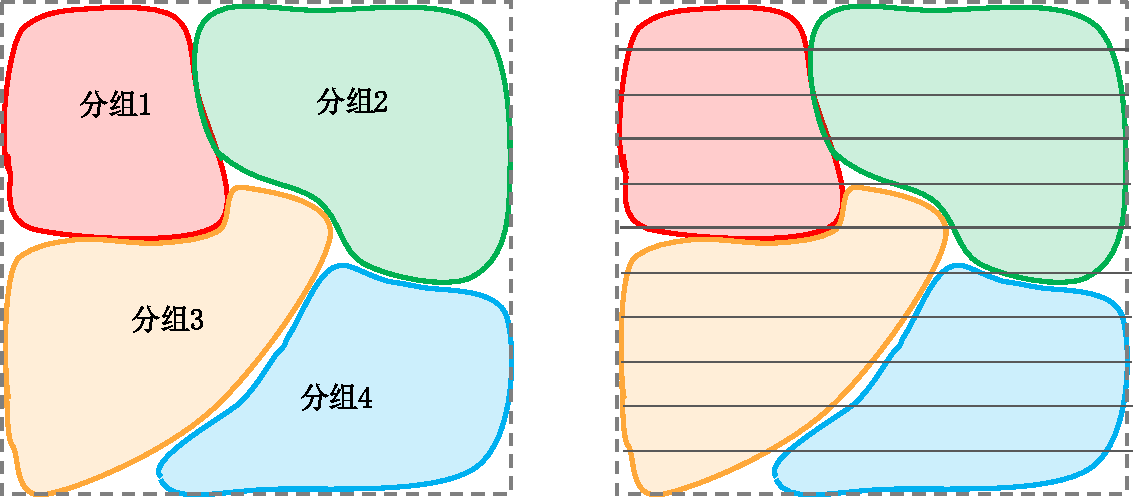
\includegraphics[width=0.95\textwidth]{image/chap04/模块化布局及合法化行分割图示.pdf}
    \caption{基于放置行边界的模块图形切分示意}
    \label{fig:chap4-legalization-row-split}
\end{figure}

\paragraph{步骤二：等高长条矩形填充与曼哈顿化重建}
在切分结果基础上，将每个高度层内的有效横向区间重建为等高长条矩形，并对相邻可合并条带进行拼接，得到满足工具约束表达的曼哈顿边界。该步骤将自由边界转化为可直接评估与迭代优化的约束表示。对应示意如图~\ref{fig:chap4-legalization-rectangle-fill} 所示。

\begin{figure}[!htbp]
    \centering
    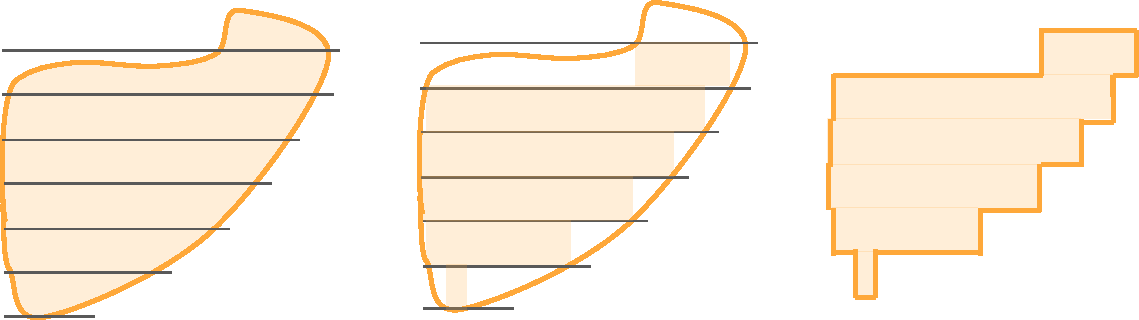
\includegraphics[width=0.95\textwidth]{image/chap04/矩形填充法构造曼哈顿图形图示.pdf}
    \caption{基于等高长条矩形的填充与曼哈顿化重建示意}
    \label{fig:chap4-legalization-rectangle-fill}
\end{figure}

\subsection{邻域操作设计}
\label{sec:chap4-neighborhood}
邻域操作决定了模拟退火在可行空间中的探索方式。考虑到\ref{sec:chap4-legalization}中给出的合法化约束，本文要求每次扰动后得到的新约束尽可能直接满足工具可接受的曼哈顿化表达，避免因额外二次合法化引入不可控偏差。此外，为了有效探索可能的解空间，邻域扰动的可行解应尽可能覆盖整个解空间。基于该原则，本文将邻域定义为如下五类原子操作：
\begin{equation}
\label{eq:chap4-neighbor-op-set}
\Omega=\left\{
\begin{aligned}
&\text{约束类型改变},\text{边微调},\text{边界拓展},\\
&\text{边界收缩},\text{整体平移}
\end{aligned}
\right\}
\end{equation}

其中，约束类型改变作用于约束类型，后四类作用于边界几何。为使探索强度与温度阶段匹配，本文将扰动强度分解为修改组数、每组修改次数和几何位移幅度三类量，并由当前温度 $T$ 动态调度。

设总分组数为 $N_g$，高低温阈值分别为 $T_h$ 和 $T_l$，则每轮参与修改的分组数可写为：
\begin{equation}
\label{eq:chap4-neighbor-group-schedule}
n_g(T)=
\begin{cases}
N_g, & T\ge T_h \\
1, & T\le T_l \\
\max\left(1,\left\lfloor 1+\dfrac{T-T_l}{T_h-T_l}(N_g-1)\right\rfloor\right), & \text{其他}
\end{cases}
\end{equation}

对于边微调与整体平移，其几何位移幅度采用线性温度映射：
\begin{equation}
\label{eq:chap4-neighbor-shift-schedule}
d_s(T)=
\begin{cases}
d_{\max}, & T\ge T_h \\
d_{\min}, & T\le T_l \\
d_{\min}+\dfrac{T-T_l}{T_h-T_l}(d_{\max}-d_{\min}), & \text{其他}
\end{cases}
\end{equation}

对于边界拓展与边界收缩等离散操作，其每组修改次数可表示为：
\begin{equation}
\label{eq:chap4-neighbor-repeat-schedule}
k_g(T)=
\begin{cases}
k_{\max}, & T\ge T_h \\
k_{\min}, & T\le T_l \\
\max\left(k_{\min},\left\lfloor k_{\min}+\dfrac{T-T_l}{T_h-T_l}(k_{\max}-k_{\min})\right\rfloor\right), & \text{其他}
\end{cases}
\end{equation}

由此可形成高温情况下大步探索，低温情况下小步进行收敛的动态施加扰动的策略。以下对五类操作分别说明。

\paragraph{操作一：约束类型改变}
该操作在单个分组约束内部修改约束类型参数，候选类型包括前文提到的三种不同强度的约束。该操作不改变几何边界，而是改变工具对该边界的约束强度，从而调整实例在区域内外的自由度。工程实现中，每轮随机选择 $n_g(T)$ 个分组执行类型扰动；温度越高，参与类型切换的分组越多，以增强全局探索能力。示意如图~\ref{fig:chap4-neighbor-type-change} 所示。

\begin{figure}[!htbp]
    \centering
    
\includegraphics[width=0.9\textwidth]{image/chap04/约束类型改变.pdf}
    \caption{邻域操作一：约束类型改变示意}
    \label{fig:chap4-neighbor-type-change}
\end{figure}

\paragraph{操作二：边微调}
该操作先将当前曼哈顿边界分解为等高长条矩形，再随机选取一个条带，随后在其左边或右边执行向内/向外微移。移动幅度由 $d_s(T)$ 控制，并在实现中额外检查矩形宽度合法性，避免出现负宽度或退化形状。该操作对应局部通道宽度的细修，能够在不破坏整体拓扑的前提下调节局部密度与连线通道。示意如图~\ref{fig:chap4-neighbor-edge-shift} 所示。

\begin{figure}[!htbp]
    \centering
    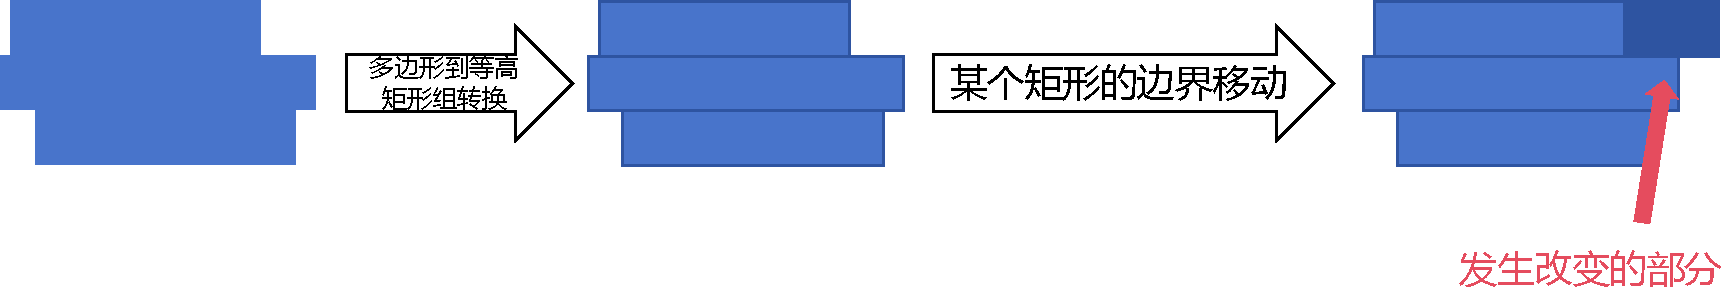
\includegraphics[width=0.9\textwidth]{image/chap04/边微调.pdf}
    \caption{邻域操作二：边微调示意}
    \label{fig:chap4-neighbor-edge-shift}
\end{figure}

\paragraph{操作三：边界拓展}
该操作在条带化表示下，仅对图形上下临边进行增量扩展：随机选择顶部或底部，在对应临边外侧新增一条等高长条矩形。新增条带通常继承临边条带的宽度与高度，从而保持放置行对齐粒度一致。其强度主要由 $k_g(T)$ 与 $n_g(T)$ 共同决定：高温阶段可在更多分组上执行多次新增，快速扩大探索覆盖范围。示意如图~\ref{fig:chap4-neighbor-add-boundary} 所示。

\begin{figure}[!htbp]
    \centering
    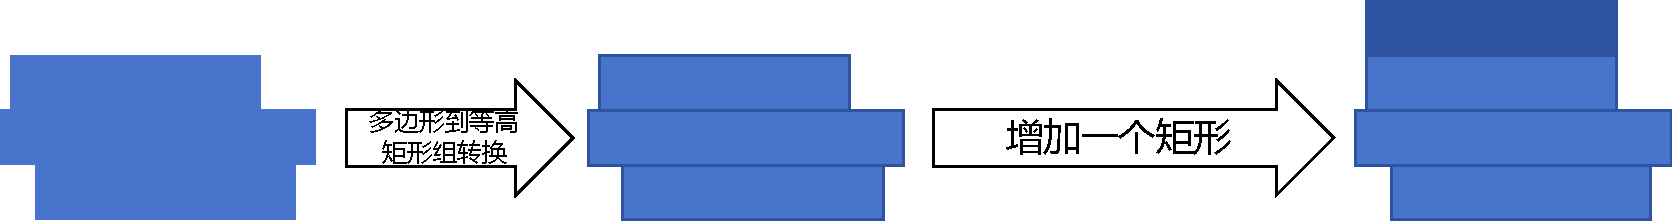
\includegraphics[width=0.9\textwidth]{image/chap04/边界拓展.pdf}
    \caption{邻域操作三：边界拓展示意}
    \label{fig:chap4-neighbor-add-boundary}
\end{figure}

\paragraph{操作四：边界收缩}
该操作与边界拓展相反，同样仅在上下临边执行离散删减：随机选择顶部或底部，移除对应临边的一条等高长条矩形。实现中设置了最小可行保护，当图形仅剩单条带时不再收缩，以避免产生空区域。该操作可用于回收过度扩展造成的冗余面积，使搜索在探索后能够回到更紧凑可行的局部。示意如图~\ref{fig:chap4-neighbor-remove-boundary} 所示。

\begin{figure}[!htbp]
    \centering
    
\includegraphics[width=0.9\textwidth]{image/chap04/边界收缩.pdf}
    \caption{邻域操作四：边界收缩示意}
    \label{fig:chap4-neighbor-remove-boundary}
\end{figure}

\paragraph{操作五：整体平移}
该操作保持边界形状不变，仅将整组多边形按上/下/左/右方向做刚体平移。其核心作用是跨区域重定位，在不改变模块内部几何结构的前提下重排模块间相对位置关系。位移幅度同样由 $d_s(T)$ 控制：高温阶段允许更大位移以提升跨区探索能力，低温阶段采用小步平移以进行精细收敛。示意如图~\ref{fig:chap4-neighbor-move-entire} 所示。

\begin{figure}[!htbp]
    \centering
    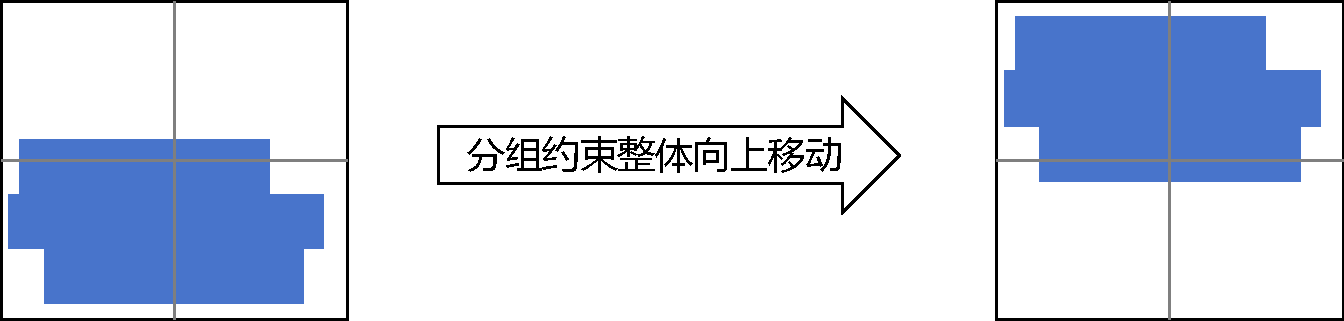
\includegraphics[width=0.9\textwidth]{image/chap04/整体平移.pdf}
    \caption{邻域操作五：整体平移示意}
    \label{fig:chap4-neighbor-move-entire}
\end{figure}

综合来看，上述五类操作分别覆盖了约束强度、局部边界、全局位置三个层面。多操作混合后，算法既能在高温阶段进行结构性探索，也能在低温阶段进行局部细修，进而提升跳出局部最优的概率。

设当前解为 $C_t$，邻域生成可写为：
\begin{equation}
\label{eq:chap4-neighbor-generate}
C_{t+1}=\Phi(C_t;\omega_t,\delta_t)
\end{equation}
其中 $\omega_t\in\Omega$ 为操作类型，$\delta_t$ 为由温度调度得到的操作强度向量（如修改组数、每组修改次数、平移幅度）。

\subsection{目标函数与接受准则}
\label{sec:chap4-objective-accept}

\subsubsection{目标函数}
\label{sec:chap4-objective}

本文方法将目标函数视为可配置项，评价函数可根据优化偏好自由指定。模拟退火流程只依赖 $J(C)$ 的相对大小，因此方法本身不依赖特定指标建模。在本章实验中，为简化问题，采用单指标线长目标：
\begin{equation}
\label{eq:chap4-objective}
J(C)=\frac{W(C)}{W_0}
\end{equation}
其中 $W(C)$ 为该约束下评估得到的总线长，$W_0$ 为初始线长，用于归一化。若任务关注其他指标，可通过替换 $J(C)$ 或扩展为多指标组合实现；算法主体与接受准则保持不变。

\subsubsection{Metropolis 接受准则}
\label{sec:chap4-metropolis}

若候选解使目标改善（$\Delta J\le 0$），则直接接受；否则按概率接受：
\begin{equation}
\label{eq:chap4-metropolis}
P_{acc}=\exp\left(-\frac{\Delta J}{T}\right)
\end{equation}
其中 $T$ 为当前温度。该机制使算法在高温阶段保持探索性，在低温阶段保持收敛性。

\subsection{多阶段退火与多轮重启策略}
\label{sec:chap4-multi-round}

为平衡探索广度与收敛稳定性，在每一阶段的模拟退火中都会根据温度动态调整扰动强度：
\begin{enumerate}
    \item 高温阶段：修改更多分组约束，增强全局探索；
    \item 中温阶段：线性降低修改范围，逐步聚焦；
    \item 低温阶段：仅修改少量分组约束，执行细粒度收敛。
\end{enumerate}





然而单轮模拟退火的常见问题是对初值敏感，如果某次模拟退火在较为前期的阶段偶然性的进入了局部最优，那么即使后续增加迭代次数，跳出局部最优的概率也会较小，这是由于布局问题的巨大搜索空间的特性导致的。为此，本章采用内层模拟退火之外，再套一层多轮模拟退火的两层结构：
\begin{enumerate}
    \item 内层迭代：标准模拟搜索过程；
    \item 外层轮次：每轮模拟退火结束后，将最优解复制为下一轮初值。
\end{enumerate}


相比于单纯增加迭代轮数的做法，多轮模拟退火可以更加有效的跳出在正常的模拟退火中偶然进入但又难以跳出的局部最优，从而在有限预算内获得更好的优化结果。与阶段性重置温度的做法相比，多轮模拟退火的区别在于重置温度的同时重置了该轮的初始解，这样可以在每轮模拟退火中都从一个新的初始解出发，增加了搜索的多样性和全局性，从而更有可能跳出局部最优，获得更好的优化结果。

该策略相当于带记忆的多次重启，可在不过度放大单轮开销的前提下提升全局搜索能力。对应伪代码如算法~\ref{alg:chap4-multi-round-sa}。
\begin{algorithm}[!htbp]
    \KwIn{初始约束 $C_0$，外层轮次 $R$，每轮迭代次数 $K$}
    \KwOut{全局最优约束 $C_{\mathrm{best}}$}
    $C_{\mathrm{best}}\leftarrow C_0$\;
    \For{$r\leftarrow 1$ \KwTo $R$}{
        $C_{\mathrm{cur}}\leftarrow C_{\mathrm{best}}$\;
        初始化温度 $T\leftarrow T_0$\;
        \For{$k\leftarrow 1$ \KwTo $K$}{
            生成邻域 $C_{\mathrm{new}}\leftarrow \mathrm{Neighbor}(C_{\mathrm{cur}},T)$\;
            调用后端工具评估 $J(C_{\mathrm{new}})$\;
            按 Metropolis 准则决定是否接受\;
            若 $J(C_{\mathrm{new}})$ 更优则更新本轮最优\;
            $T\leftarrow \mathrm{cooling}(T)$\;
        }
        用本轮最优更新 $C_{\mathrm{best}}$\;
    }
    \caption{多轮细粒度约束优化流程}
    \label{alg:chap4-multi-round-sa}
\end{algorithm}

\subsection{几何合法性检查机制}
\label{sec:chap4-feasibility-guard}

模拟退火邻域扰动可能生成几何上不可接受的约束形态。为避免非法候选污染搜索过程并进入高开销的后端评估，本章在工程实现中引入几何合法性检查机制，并仅保留满足检查条件的候选约束。检查重点包括：
\begin{enumerate}
    \item 基本几何有效性检查：确认边界宽度与高度非负、顶点序列完整且无异常重复；
    \item 多边形结构一致性检查：对连续共线点执行去冗余处理，减少工具解析歧义；
    \item 几何非法形态检查：识别自交、异常折返或退化形状等不可接受边界。
\end{enumerate}

\begin{figure}[!htbp]
    \centering
    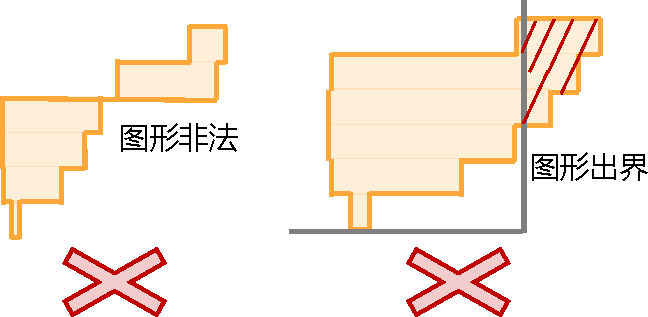
\includegraphics[width=0.8\textwidth]{image/chap04/几何非法示例.pdf}
    \caption{几何非法示例与合法性检查目标}
    \label{fig:chap4-geometry-illegal-example}
\end{figure}

图~\ref{fig:chap4-geometry-illegal-example}给出了典型几何非法示例。对于未通过检查的候选约束，本文不进入后端评估，而是直接丢弃并重新执行随机扰动，直至生成满足几何合法性要求的候选。该机制本质上减少了无效评估比例。在工具驱动型优化中，减少无效评估往往比提升单次候选质量更关键，因为其直接影响总预算利用效率。

\subsection{遗传算法在模块级布局优化中的应用尝试}
\label{sec:chap4-ga-application}

在设计算法阶段，除了模拟退火算法，遗传算法也在调研范围之内。和模拟退火算法一样，遗传算法也是一种经典的优化方法，为评估遗传算法路线在本问题中的可行性，本文在研究阶段也构建了基于遗传算法的原型。该方法将分组约束配置视为可进化个体，个体中包含分组边界几何与约束强度信息；通过完整后端流程评估其质量，以线长等指标作为适应度反馈。

在模块级布局约束优化中，遗传算法可按以下步骤应用：
\begin{enumerate}
    \item 个体编码与初始化：将初始模块级布局约束映射为若干候选个体，并通过随机扰动扩充初始种群，形成多起点搜索；
    \item 真实指标评估：对每个个体执行完整评估流程，提取线长、通孔与运行时间等指标，计算适应度；
    \item 父代选择与精英保留：通过竞争选择保留高质量个体，并将最优个体直接继承到下一代，避免优质解丢失；
    \item 约束重组：从两个父代中重组部分分组约束，形成新候选，以扩大搜索多样性；
    \item 变异扰动：对候选解执行约束类型改变、边微调、边界扩展、边界收缩与整体平移等操作，在局部空间中引入新结构；
    \item 分阶段强度调度：随着代数增加，逐步降低变异范围与扰动幅度，实现由全局探索向局部收敛过渡。
\end{enumerate}
遗传算法的整体流程如图~\ref{fig:chap4-ga-workflow} 所示：

\begin{figure}[!htbp]
    \centering
    \begin{tikzpicture}[
        node distance=7mm and 16mm,
        block/.style={rectangle, rounded corners, draw=black, thick, align=center, minimum width=4.2cm, minimum height=8.5mm, fill=gray!8},
        decision/.style={diamond, draw=black, thick, align=center, aspect=2.2, inner sep=1.2pt, fill=gray!8},
        line/.style={-{Stealth[length=2.2mm]}, thick}
    ]
        \node[block] (init) {个体编码与初始化};
        \node[block, below=of init] (eval) {真实指标评估};
        \node[block, below=of eval] (select) {父代选择与精英保留};
        \node[block, below=of select] (cross) {约束重组};
        \node[block, below=of cross] (mut) {变异扰动};
        \node[block, below=of mut] (schedule) {分阶段强度调度};
        \node[decision, below=of schedule] (stop) {达到终止条件？};
        \node[block, below=of stop] (out) {输出当前最优约束};

        \draw[line] (init) -- (eval);
        \draw[line] (eval) -- (select);
        \draw[line] (select) -- (cross);
        \draw[line] (cross) -- (mut);
        \draw[line] (mut) -- (schedule);
        \draw[line] (schedule) -- (stop);
        \draw[line] (stop) -- node[right]{是} (out);
        \draw[line] (stop.west) -- ++(-2.2,0) node[above,pos=0.4]{否} |- (eval.west);
    \end{tikzpicture}
    \caption{遗传算法在模块级布局约束优化中的流程示意}
    \label{fig:chap4-ga-workflow}
\end{figure}

上述流程说明，遗传算法能够在早期快速覆盖较大搜索空间，具备较强的全局探索潜力；但其代价是每一代都需要评估多个候选解，计算开销与评估预算高度相关。

\subsection{模拟退火与遗传算法的差异及优劣分析}
\label{sec:chap4-sa-vs-ga}

基于上述实现，可将模拟退火与遗传算法的差异归纳为以下几点：
\begin{enumerate}
    \item 搜索组织方式不同：模拟退火沿单解轨迹逐步演化，遗传算法并行维护群体并通过群体多样性扩展搜索范围；
    \item 新解产生机制不同：模拟退火依赖邻域扰动与概率接受；遗传算法依赖选择、重组与变异；
    \item 开销结构不同：若种群规模为 $P$、迭代代数为 $G$、每代精英数为 $E$，遗传算法评估次数近似为

\begin{equation}
\label{eq:chap4-ga-eval-count}
N_{eval}^{GA}\approx N_0 + G\cdot(P-E)
\end{equation}

其中 $N_0$ 为初始种群评估开销；而模拟退火评估次数通常可写为

\begin{equation}
\label{eq:chap4-sa-eval-count}
N_{eval}^{SA}\approx R\cdot K
\end{equation}

其中 $R$ 为外层轮次、$K$ 为每轮迭代数。对于评估代价昂贵的问题，模拟退火更便于按预算精细控制；
    \item 收敛行为不同：遗传算法更强调全局多样性，模拟退火更强调局部连续改进与稳定收敛。
\end{enumerate}

从理论分析的角度，遗传算法的优势在于全局探索能力强、对初值依赖相对较弱；不足在于参数耦合度高、评估开销大、收敛速度对种群配置敏感。模拟退火的优势在于预算可控、实现简洁、在较优初值附近易获得稳定增量收益；不足在于单轮搜索可能陷入局部最优。本文通过多轮重启与动态强度调度，部分缓解了模拟退火的局部最优风险。

但综合考虑质量收益与计算效率的权衡，遗传算法在该场景下未必能表现出显著更强的优化收益，但其整体运行速度明显慢于模拟退火。其核心瓶颈在于群体方法需要反复评估大量候选解，而每次评估都依赖高代价后端流程。

由式\ref{eq:chap4-ga-eval-count} 与\ref{eq:chap4-sa-eval-count} 的评估次数分析为基础，假设每次评估的平均开销为 $C_{eval}$，则遗传算法的总评估开销约为 $C_{eval}\cdot N_{eval}^{GA}$，而模拟退火的总评估开销约为 $C_{eval}\cdot N_{eval}^{SA}$。在实际工程中，若 $P$ 和 $G$ 较大，遗传算法的评估造成的时间开销远超模拟退火。


因此，在评估时间成本高、追求稳定改进两个目的的权衡下，选择模拟退火作为本章主方法具有一定的优势。%并且，本文将会在后续实验测试章节中对两种方法进行对比测试。

\section{实验测试与结果分析}
\label{sec:chap4-exp}

\subsection{实验目标、对比策略与测试基准}
\label{sec:chap4-exp-goal-benchmark}

围绕本章提出的多段模拟退火细粒度优化流程，实验测试聚焦以下两个核心问题：
\begin{enumerate}
    \item 对于一个模块级布局规划，多段模拟退火优化前后是否能够改善关键指标；
    \item 模拟退火搜索过程对模块布局约束的引导变化是否具有可解释性，并能够在典型案例上形成可视化证据。
\end{enumerate}

由于当前阶段缺乏可直接对齐的同类型公开对比方法，本文采用同流程前后对比作为主评估策略：以优化前结果作为基线，以优化后结果作为对照，比较二者在相同评估链路下的指标变化。该策略能够在现有工程条件下较真实地反映本章方法的增量收益。

本文实验的测试环境为Centos7系统，并基于 Cadence Innovus 20.01 版本完成后端流程测试和指标反馈。其中，Cadence Innovus为后端物理设计环节的知名工具，具有极高的通用性，通过Innovus完成运行从读取网表到完成布局的全过程并反馈关键指标给模拟退火程序控制程序，具有较高的可信度与实用价值。

整个优化流程由一个多段模拟退火程序控制，该程序主要功能有两个，首先是基于邻域设定对模块级布局约束进行随机扰动，其次是根据 Innovus 执行后端流程的指标反馈，按接受准则决定是否保留该扰动。由于多段模拟退火控制程序本身不执行重型后端计算，仅承担扰动生成与接受判定，单次开销远小于 Innovus 评估流程开销。在实验统计中，可近似认为总运行时间主要由 Innovus 后端评估流程贡献，模拟退火脚本自身时间开销可忽略不计。


测试基准方面，本节样例来自 ITC'99 基准集。当前用于实验的样例基础信息如表~\ref{tab:chap4-itc99-benchmark} 所示，覆盖了从小规模到中大规模的多个 case，可用于观察算法在不同规模下的行为差异。

\begin{table}[!htbp]
    \centering
    \caption{ITC'99测试样例基础信息}
    \label{tab:chap4-itc99-benchmark}
    \small
    \setlength{\tabcolsep}{6pt}
    \renewcommand{\arraystretch}{1.08}
    \begin{tabular}{l c c c}
        \hline
        测试用例 & 实例数 & 模块数 & 线网数 \\
        \hline
        \texttt{b11} & 0.3k & 4  & 0.3k \\
        \texttt{b12} & 0.7k & 4  & 0.7k \\
        \texttt{b13} & 0.2k & 4  & 0.2k \\
        \texttt{b14} & 2.2k & 8  & 2.3k \\
        \texttt{b15} & 4.1k & 8  & 4.2k \\
        \texttt{b17} & 12.7k & 8  & 12.8k \\
        \texttt{b18} & 29.1k & 12 & 29.4k \\
        \texttt{b19} & 56.7k & 18 & 57.0k \\
        \texttt{b20} & 4.8k & 8  & 4.9k \\
        \texttt{b21} & 4.8k & 8  & 4.8k \\
        \texttt{b22} & 7.0k & 8  & 7.1k \\
        \hline
    \end{tabular}
\end{table}

\subsection{模拟退火优化前后对比}
\label{sec:chap4-exp-before-after}

为清晰展示多段模拟退火的优化作用，本小节对比优化前后关键指标的变化情况。对比基准为未经过模拟退火优化的模块级布局约束引导下的布局结果。对每个测试样例，分别记录优化前与优化后的关键指标：

本文的多轮模拟退火策略如下：每一轮模拟退火进行 20 次迭代，每一轮模拟退火的起点为前一轮的最优解，若连续三轮无任何指标改善则终止多轮模拟退火布局优化。

表~\ref{tab:chap4-sa-before-after} 列出了每个测试样例的最优迭代次数、并对比优化前后线长、通孔数，并检查了最差负时序裕量（Worst Negative Slack, WNS）总负时序裕量（Total Negative Slack, TNS） ，还计算了线长改善率。可以看到，在所有测试样例中，经过多段模拟退火优化后，线长均有不同程度的改善，平均改善率达到 3.86\%。同时，通孔数在大多数样例中保持稳定，表明了优化的有效性。此外，最差负时序裕量和总负时序裕量在优化后均满足时序设计要求，未出现新的时序违规。
\begin{table}[!htbp]
    \centering
    \caption{多段模拟退火优化前后关键指标对比}
    \label{tab:chap4-sa-before-after}
    \small
    \setlength{\tabcolsep}{4.2pt}
    \renewcommand{\arraystretch}{1.05}
    \resizebox{\textwidth}{!}{
        \begin{tabular}{l c c c c c c c c}
            \toprule
            \multirow{2}{*}{测试用例} & \multirow{2}{*}{最优迭代次} & \multicolumn{2}{c}{线长} & \multicolumn{2}{c}{通孔数} & \multirow{2}{*}{WNS(后)/ns} & \multirow{2}{*}{TNS(后)/ns} & \multirow{2}{*}{线长改善率/\%} \\
            \cmidrule(lr){3-4} \cmidrule(lr){5-6}
            & & 优化前 & 优化后 & 优化前 & 优化后 & & & \\
            \midrule
            \texttt{b11} & 26  & 441.210   & 425.407   & 2467   & 2476   & 3.837 & 0.000 & 3.58 \\
            \texttt{b12} & 74  & 1209.134  & 1194.521  & 7006   & 7032   & 3.844 & 0.000 & 1.21 \\
            \texttt{b13} & 70  & 251.079   & 245.889   & 1820   & 1841   & 4.486 & 0.000 & 2.07 \\
            \texttt{b14} & 36  & 4323.798  & 4246.052  & 22103  & 21873  & 0.415 & 0.000 & 1.80 \\
            \texttt{b15} & 108 & 10318.628 & 9903.889  & 43476  & 42929  & 1.644 & 0.000 & 4.02 \\
            \texttt{b17} & 81  & 34575.863 & 32852.170 & 135612 & 132817 & 1.923 & 0.000 & 4.99 \\
            \texttt{b18} & 242 & 77466.022 & 74950.343 & 306887 & 302196 & 0.110 & 0.000 & 3.25 \\
            \texttt{b19} & 78  & 161974.563 & 152036.894 & 607661 & 600117 & 0.855 & 0.000 & 6.14 \\
            \texttt{b20} & 30  & 10708.252 & 10222.663 & 49164  & 48672  & 0.067 & 0.000 & 4.53 \\
            \texttt{b21} & 16  & 10961.191 & 10552.232 & 48474  & 47674  & 0.332 & 0.000 & 3.73 \\
            \texttt{b22} & 84  & 16671.322 & 15484.965 & 73020  & 70561  & 0.180 & 0.000 & 7.12 \\
            \midrule
            平均比例 & -- & 1.000 & 0.961 & 1.000 & 0.990 & -- & -- & 3.86 \\
            \bottomrule
        \end{tabular}
    }
\end{table}

\subsection{典型案例布局引导约束可视化分析}
\label{sec:chap4-exp-case-visual}

本文选取 \texttt{b20}、\texttt{b21} 与 \texttt{b22} 三个测试用例，并分别展示优化前后模块级布局规划以及实际布局结果可视化图。图中包含若干模块，不同模块以不同颜色区分；其中颜色相对较深的框表示模块级布局规划的约束边界，也即本章算法所处理的对象。

从图中可观察到，随着模拟退火对引导约束形状进行细粒度调整，模块的空间分布也随之发生细粒度的变化。这表明引导约束能够有效参与布局优化过程。结合表~\ref{tab:chap4-sa-before-after} 的结果（\texttt{b20} 线长改善 4.53\%，\texttt{b21} 线长改善 3.73\%，\texttt{b22} 线长改善 7.12\%），实验测试说明这种由约束引导带来的布局变化能够转化为有效的质量收益。

\begin{figure}[!htbp]
    \centering
    \begin{minipage}[t]{0.4\textwidth}
        \centering
        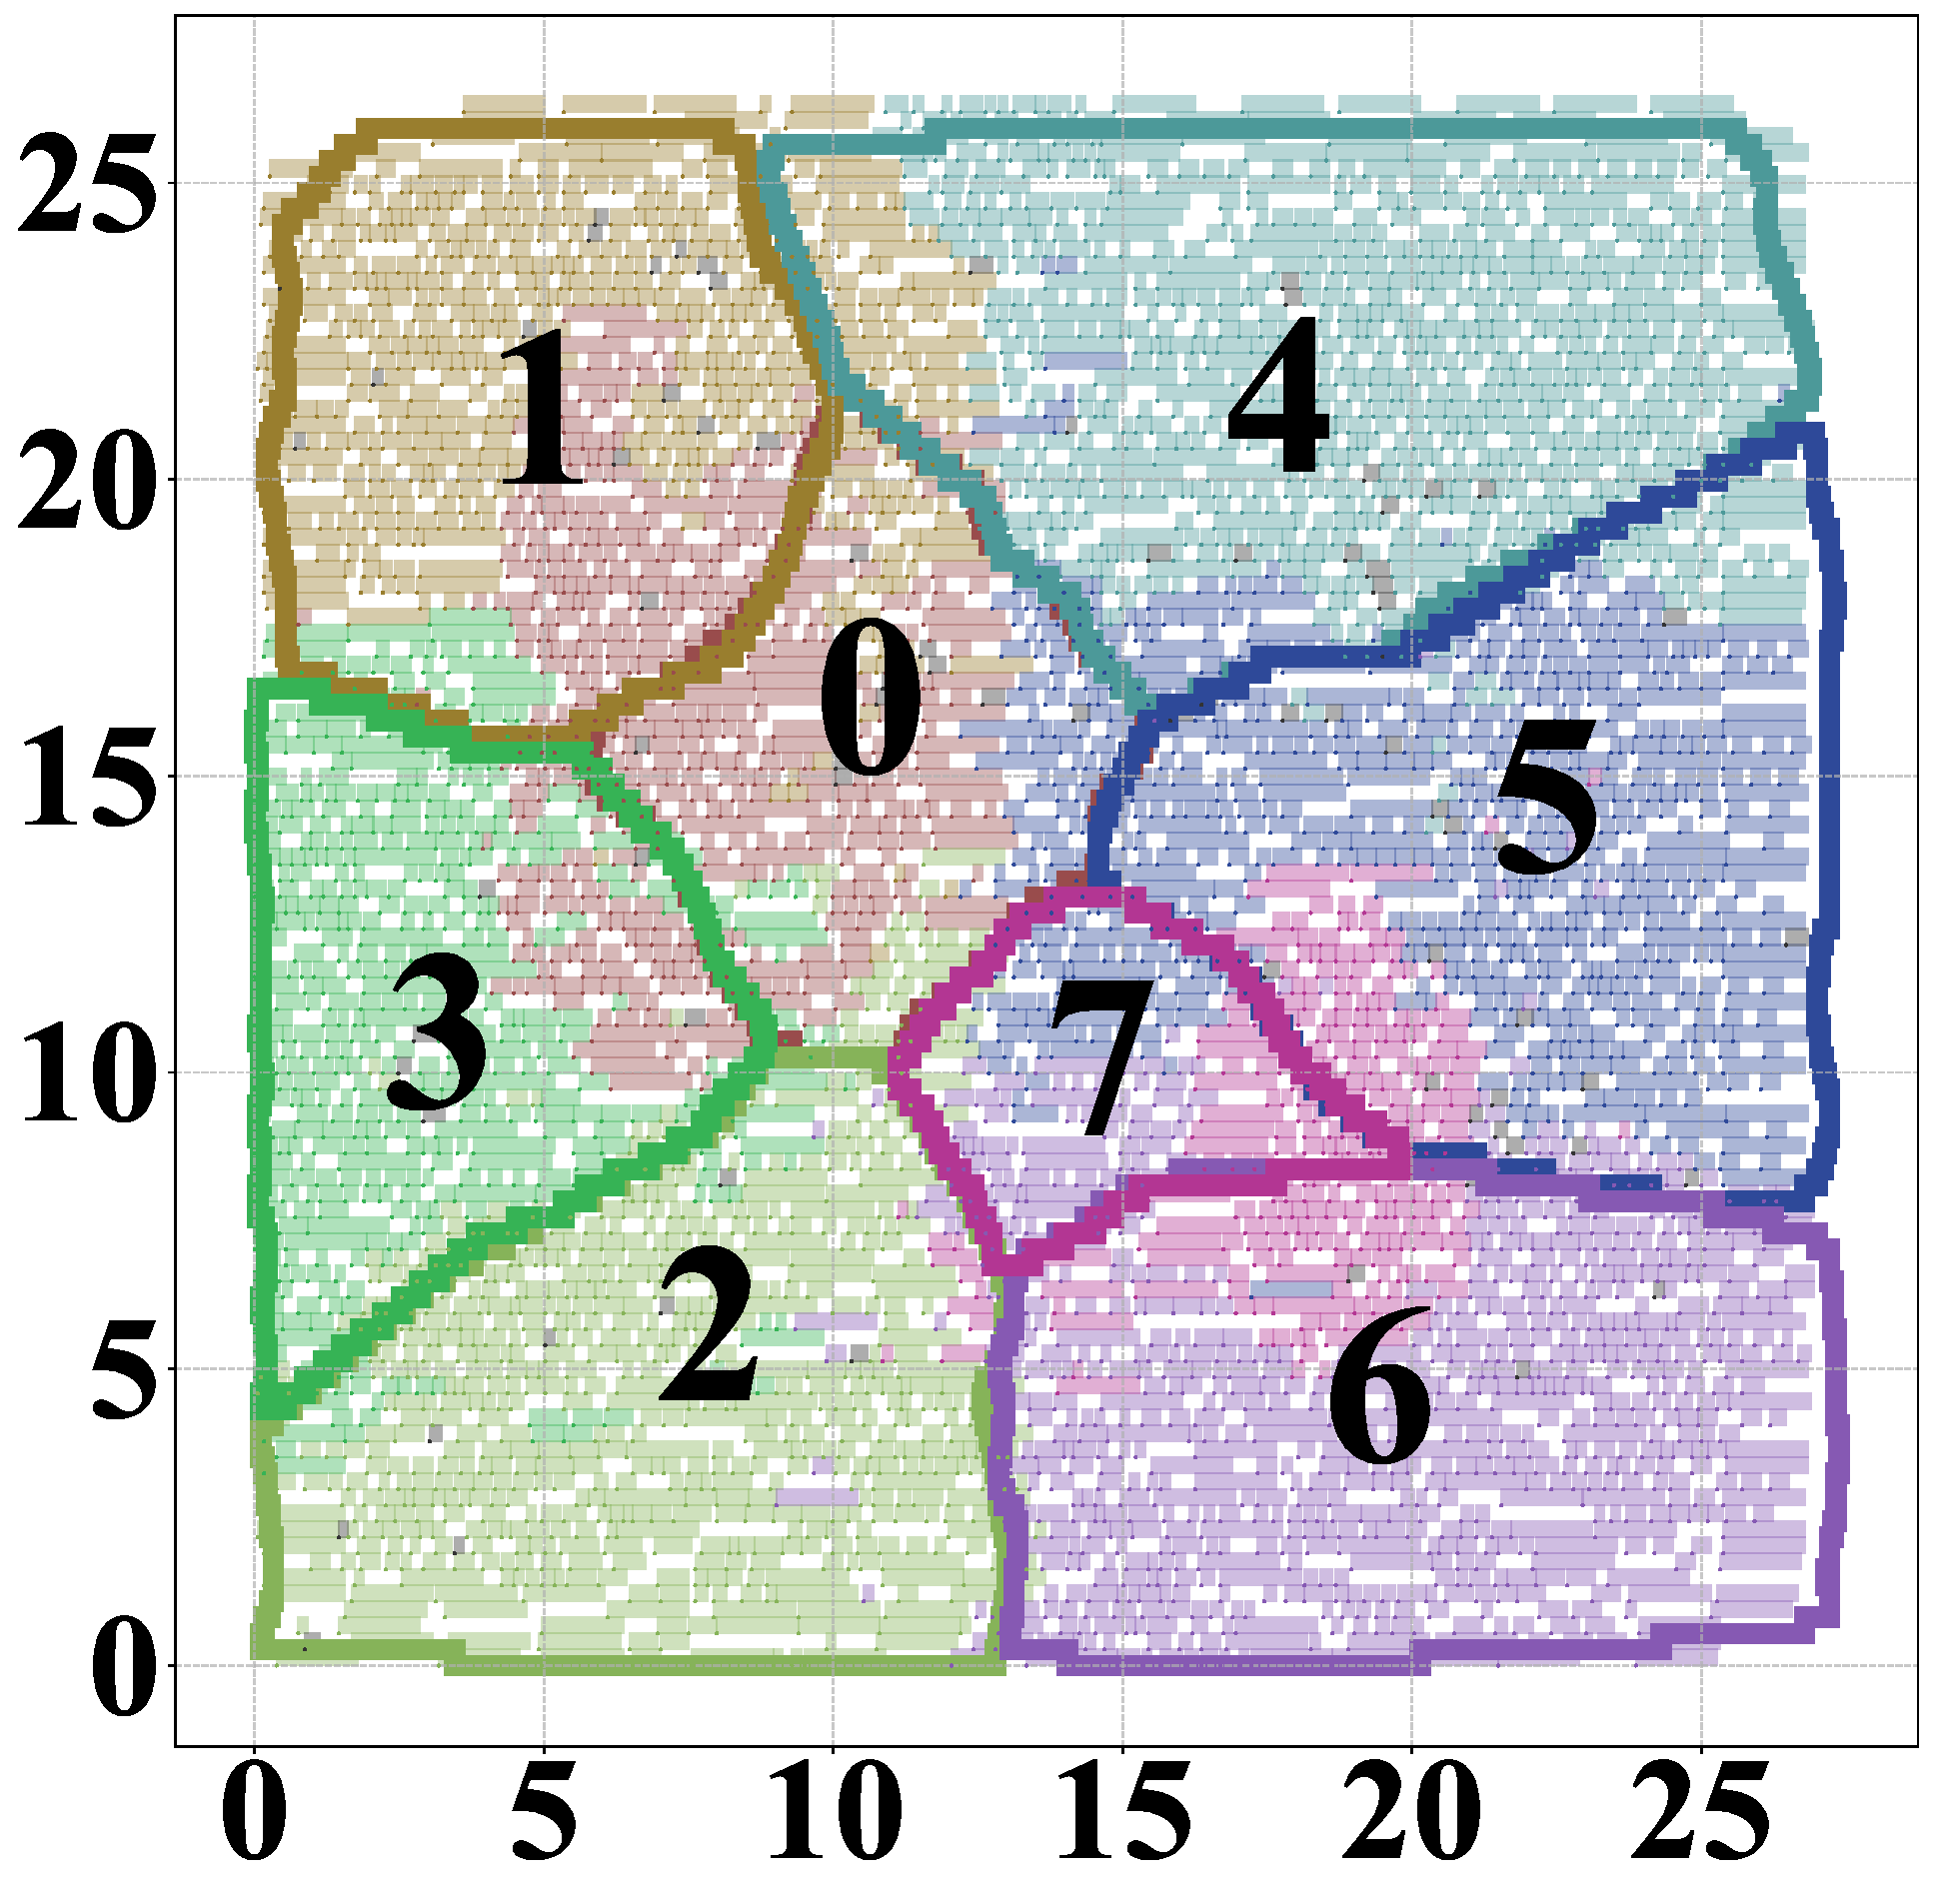
\includegraphics[width=\textwidth]{image/chap04/b20_iter0.pdf}
        \\
        \small (a) \texttt{b20} 优化前
    \end{minipage}
    \hfill
    \begin{minipage}[t]{0.4\textwidth}
        \centering
        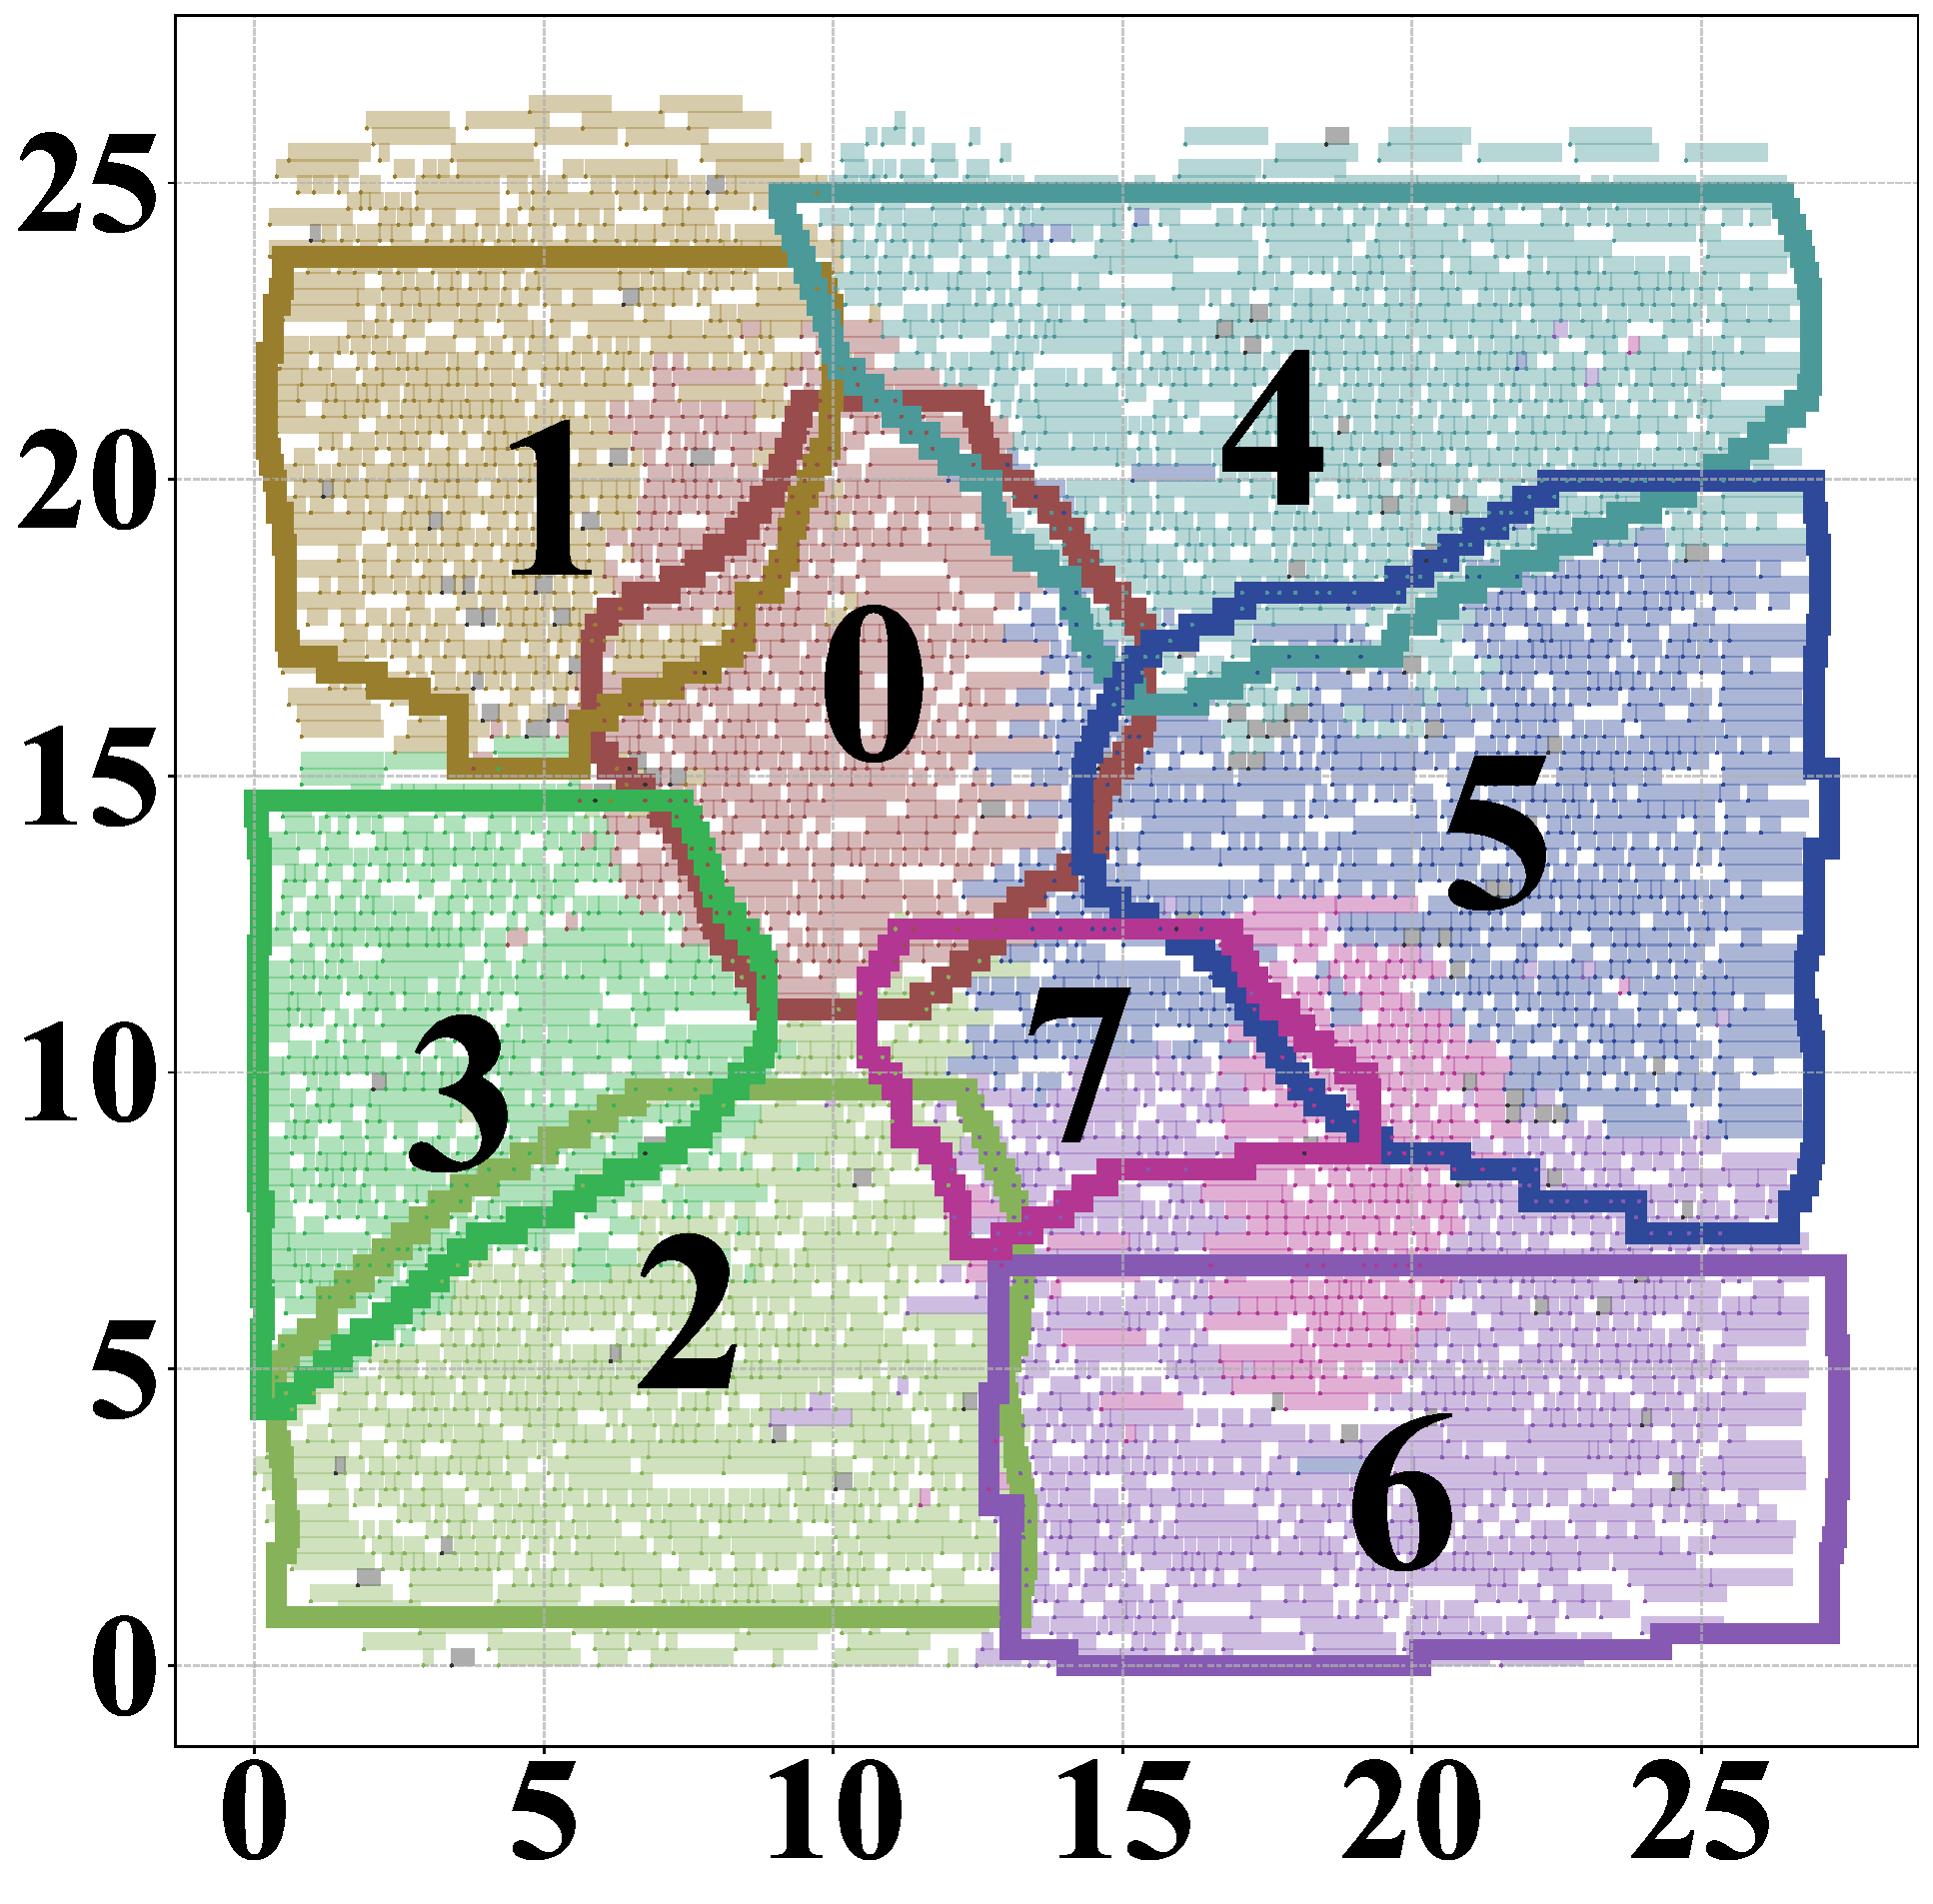
\includegraphics[width=\textwidth]{image/chap04/b20_iter30.pdf}
        \\
        \small (b) \texttt{b20} 优化后（最优迭代次 30）
    \end{minipage}
    \caption{\texttt{b20} 优化前后布局引导对比}
    \label{fig:chap4-case-b20-before-after}
\end{figure}

\begin{figure}[!htbp]
    \centering
    \begin{minipage}[t]{0.4\textwidth}
        \centering
        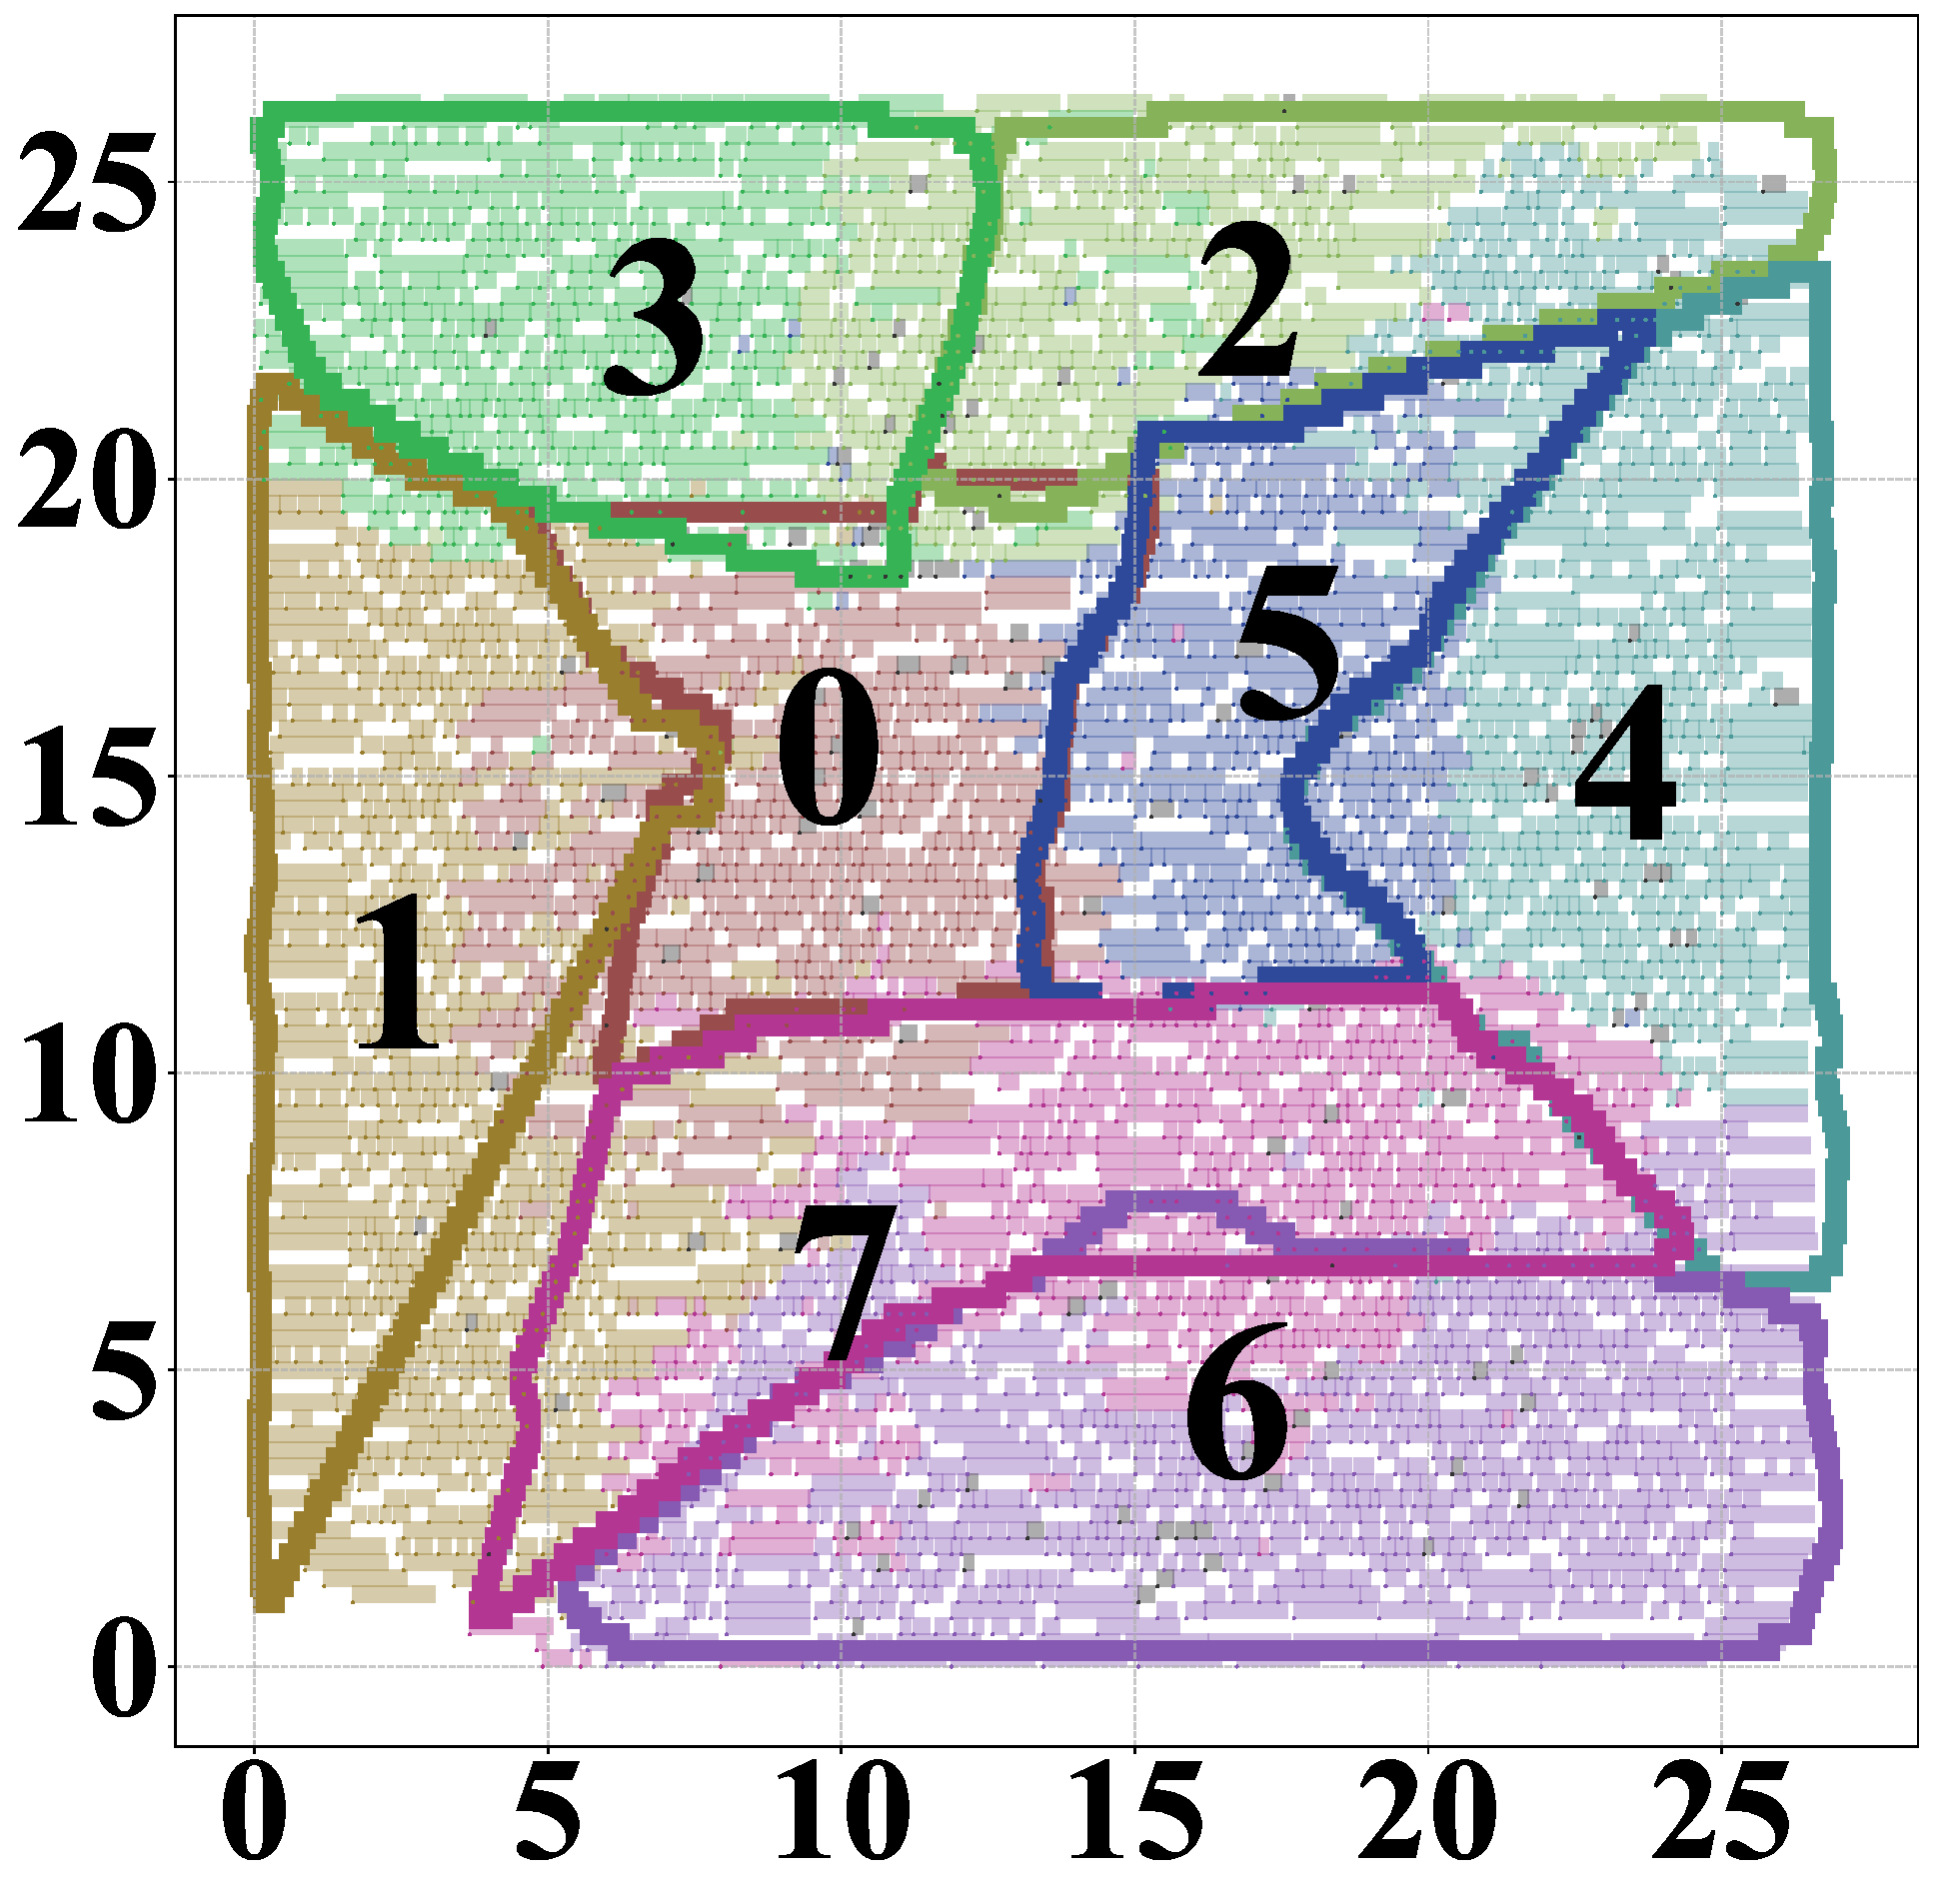
\includegraphics[width=\textwidth]{image/chap04/b21_iter0.pdf}
        \\
        \small (a) \texttt{b21} 优化前
    \end{minipage}
    \hfill
    \begin{minipage}[t]{0.4\textwidth}
        \centering
        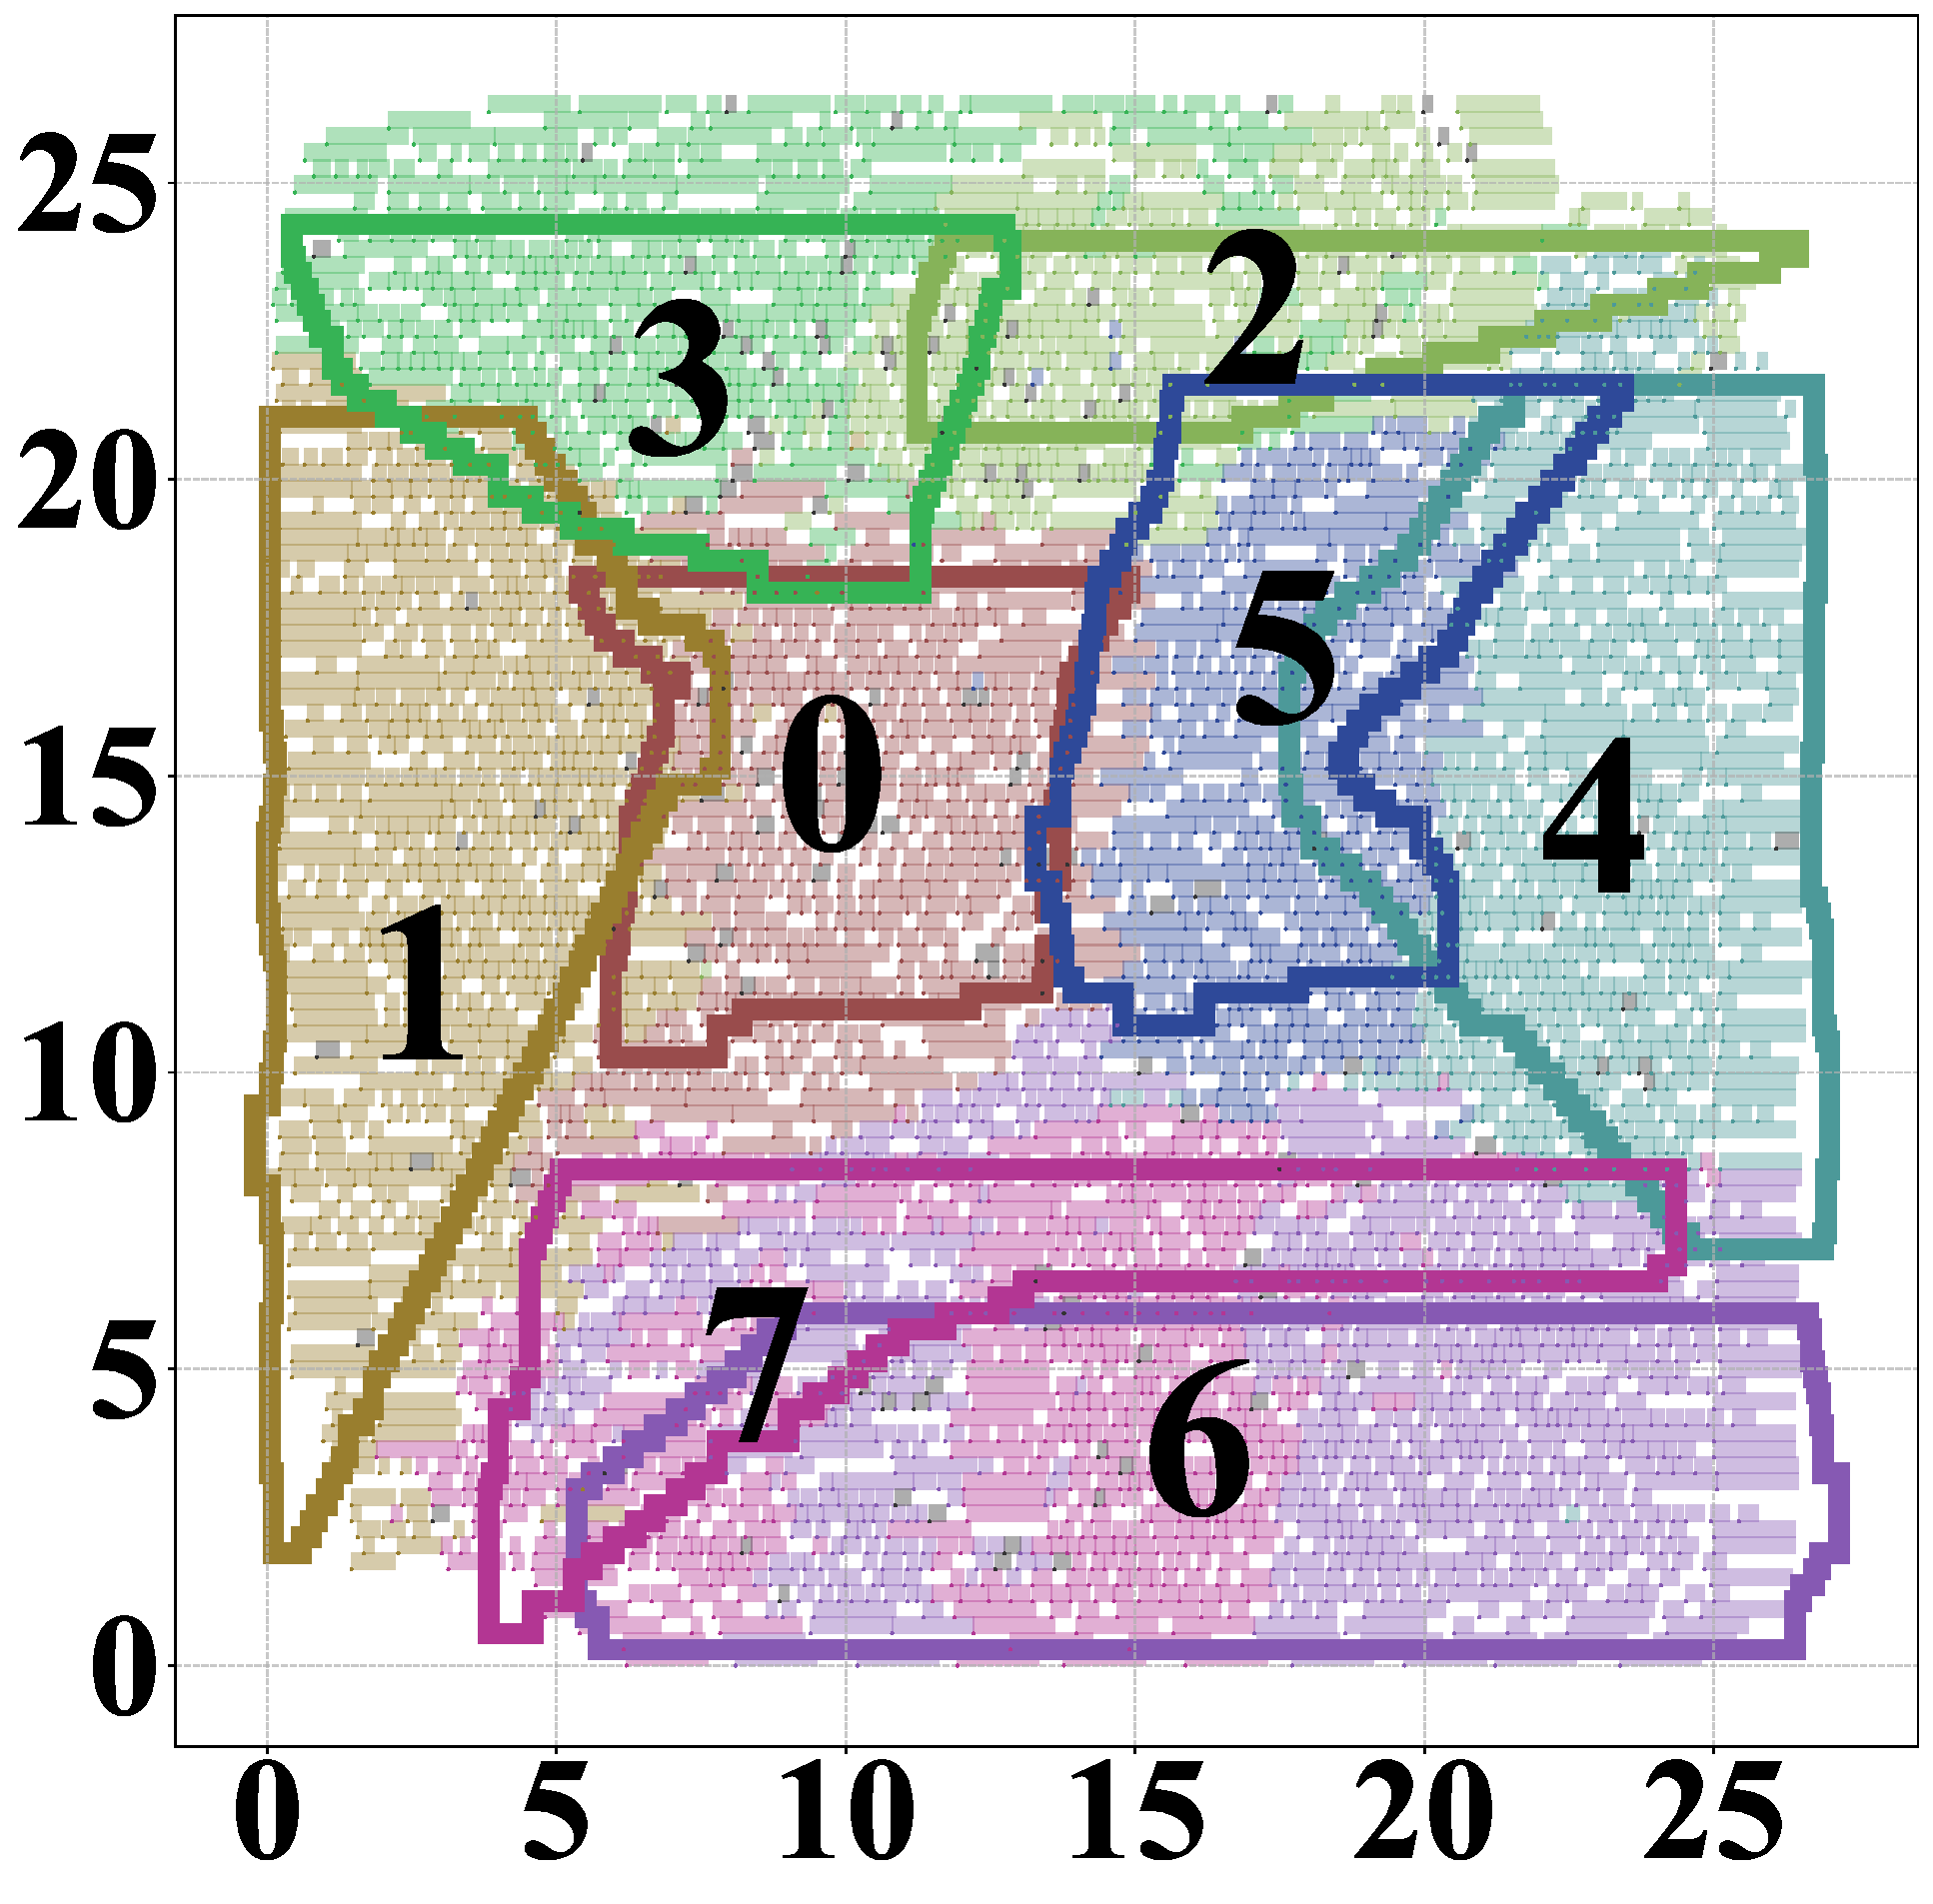
\includegraphics[width=\textwidth]{image/chap04/b21_iter16.pdf}
        \\
        \small (b) \texttt{b21} 优化后（最优迭代次 16）
    \end{minipage}
    \caption{\texttt{b21} 优化前后布局引导对比}
    \label{fig:chap4-case-b21-before-after}
\end{figure}

\begin{figure}[!htbp]
    \centering
    \begin{minipage}[t]{0.4\textwidth}
        \centering
        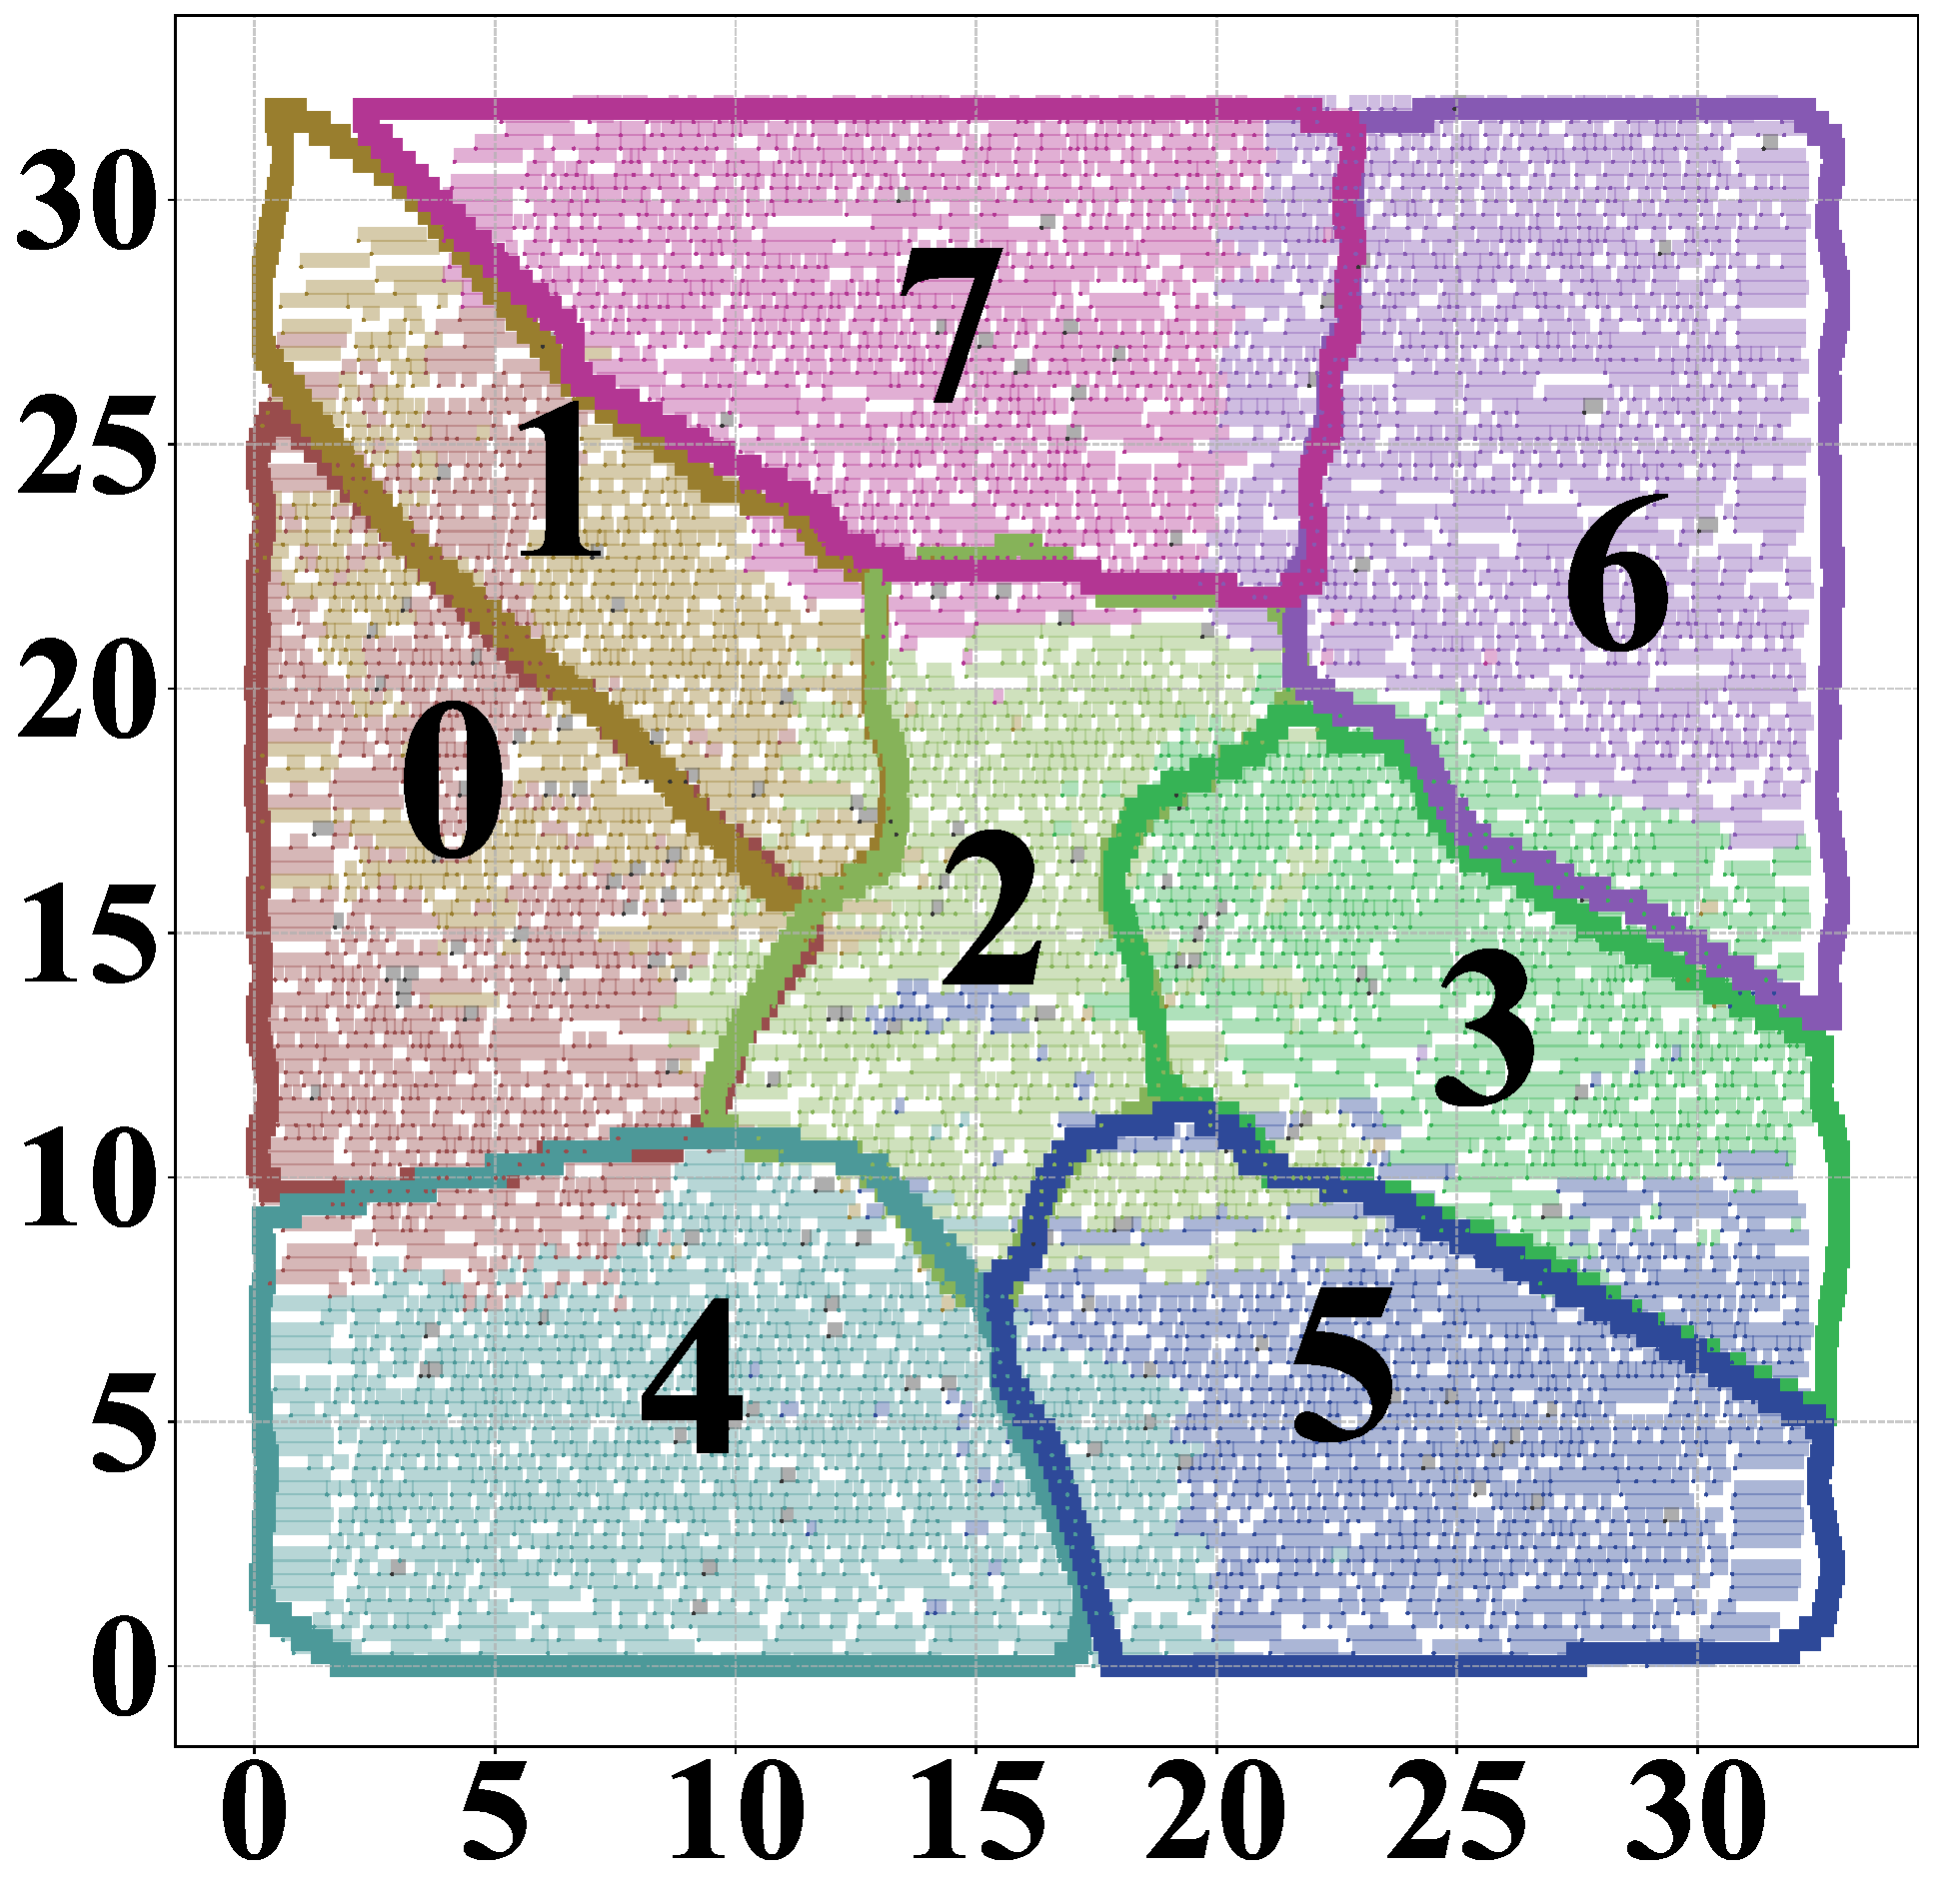
\includegraphics[width=\textwidth]{image/chap04/b22_iter0.pdf}
        \\
        \small (a) \texttt{b22} 优化前
    \end{minipage}
    \hfill
    \begin{minipage}[t]{0.4\textwidth}
        \centering
        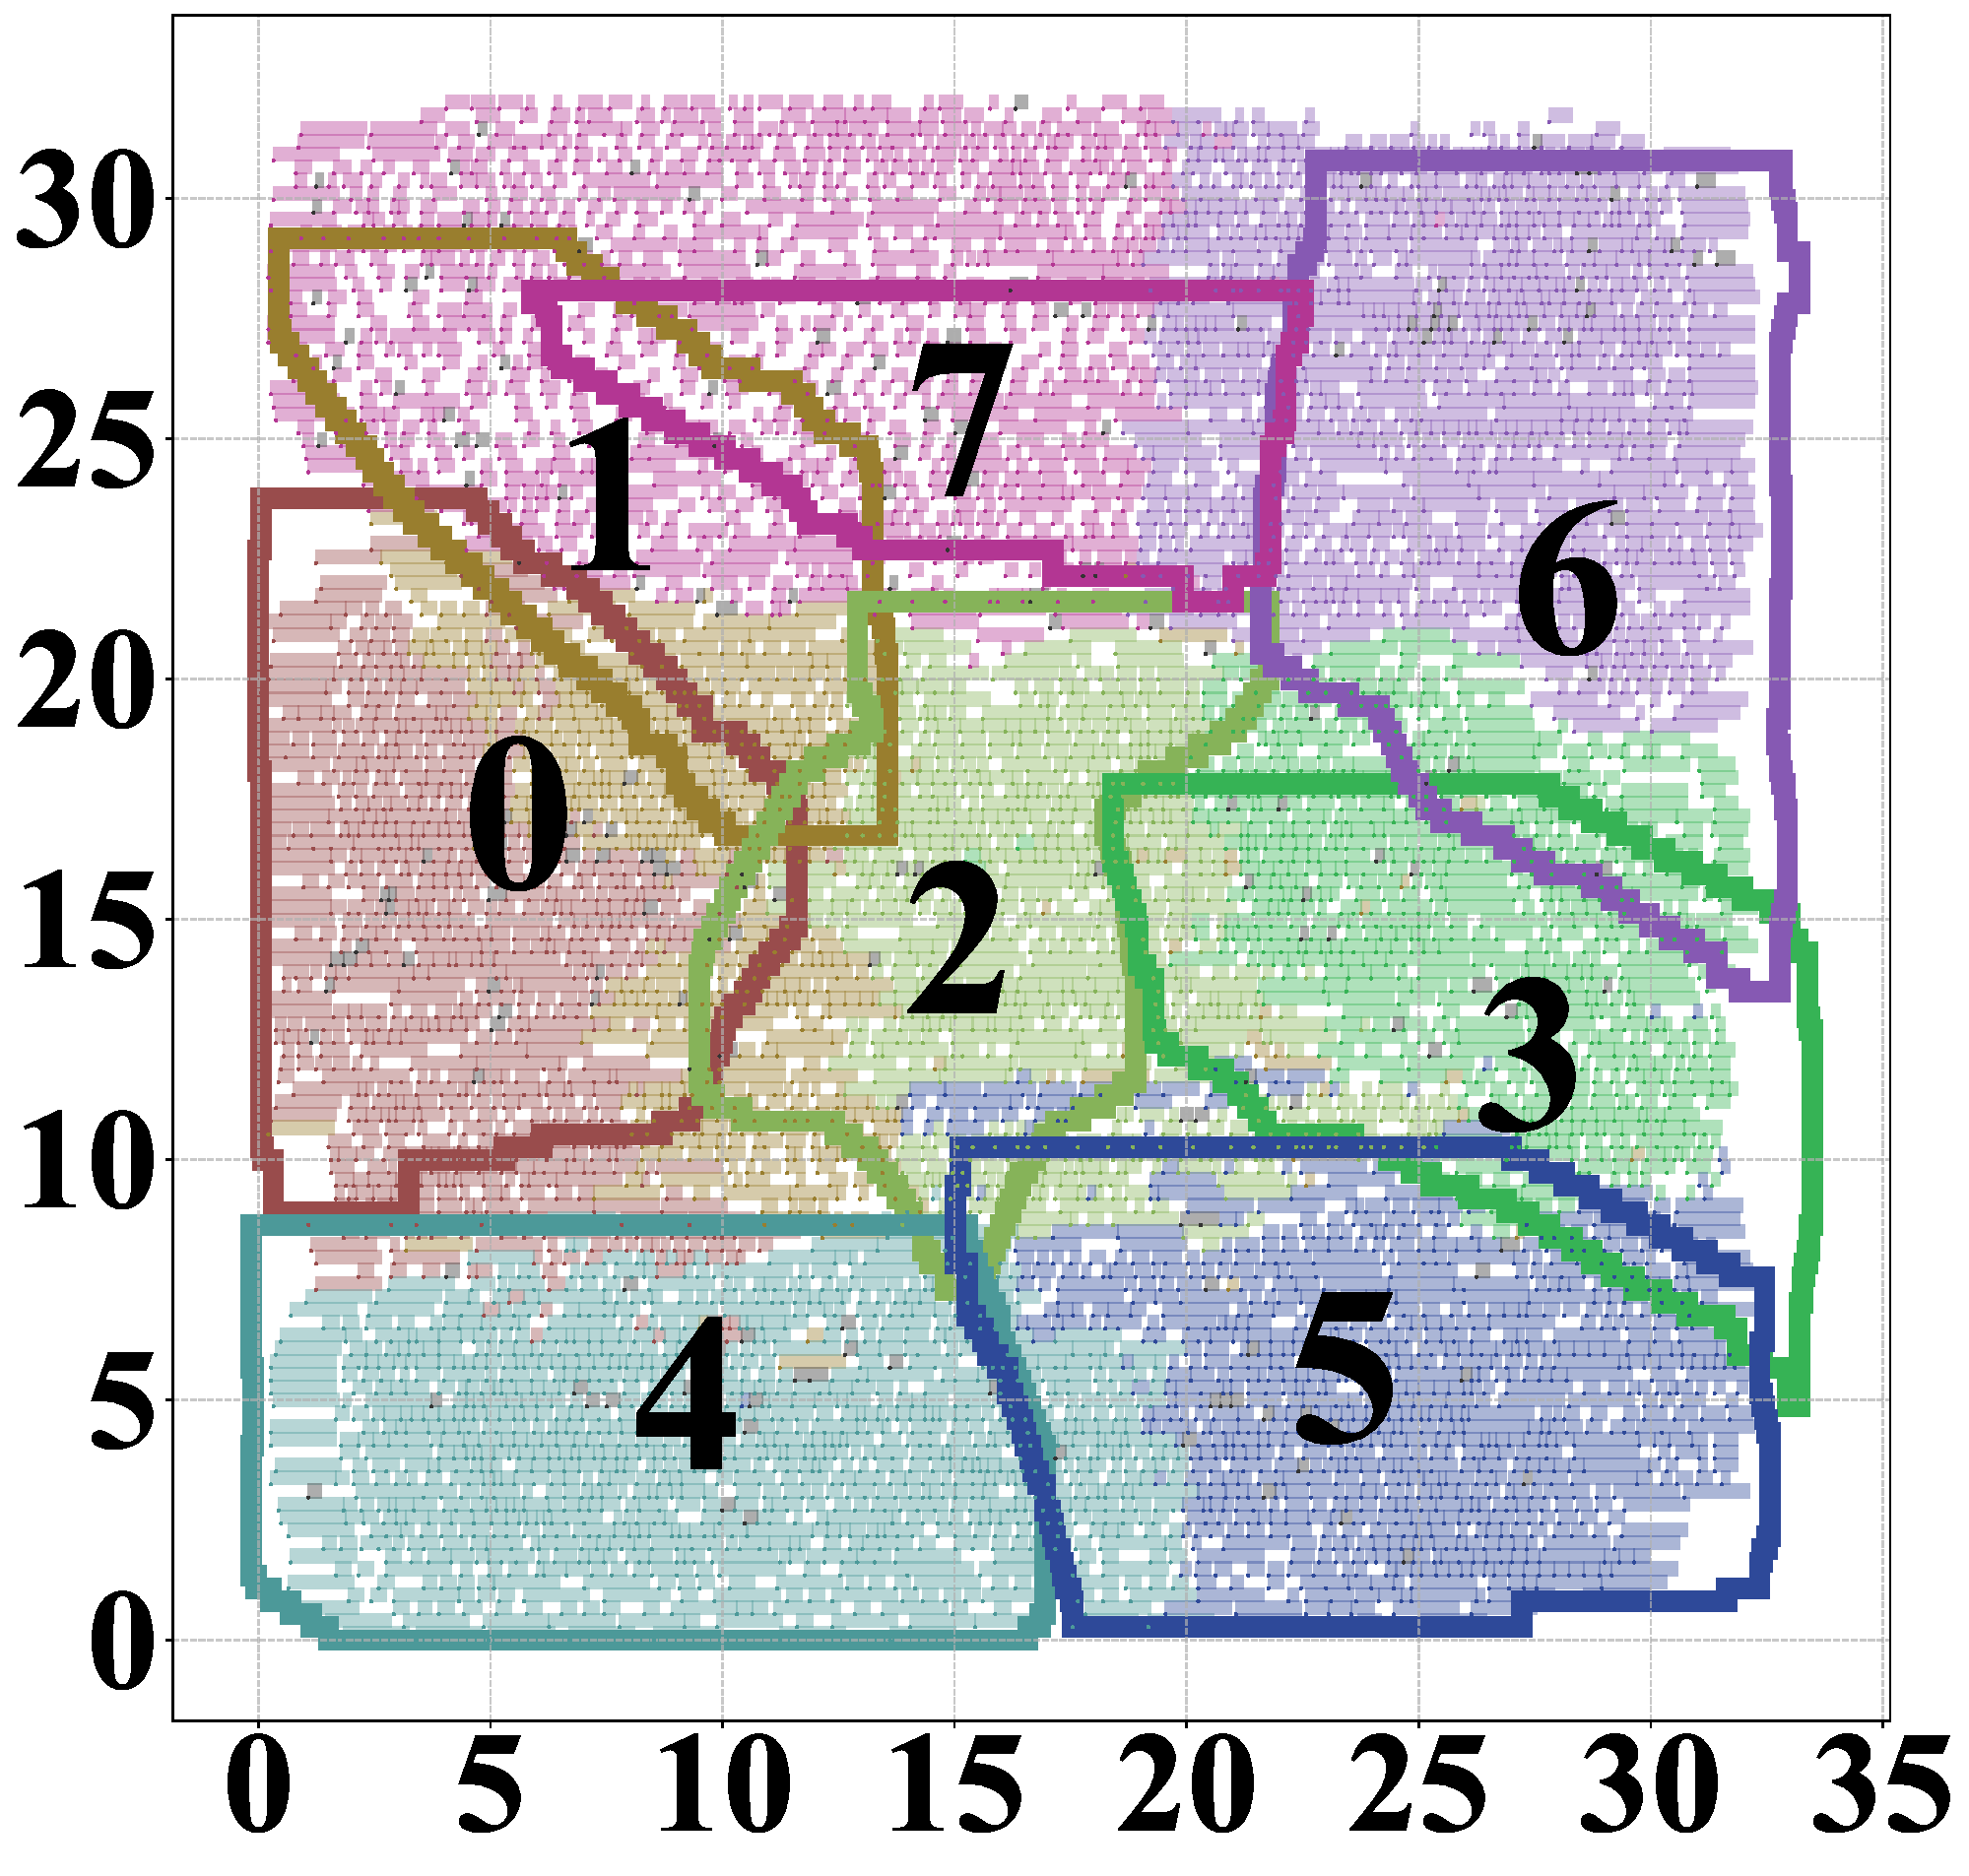
\includegraphics[width=\textwidth]{image/chap04/b22_iter84.pdf}
        \\
        \small (b) \texttt{b22} 优化后（最优迭代次 84）
    \end{minipage}
    \caption{\texttt{b22} 优化前后布局引导对比}
    \label{fig:chap4-case-b22-before-after}
\end{figure}

\subsection{多段模拟退火优化曲线分析（\texttt{b20}）}
\label{sec:chap4-exp-sa-curve-b20}

为进一步展示多段模拟退火在真实优化过程中的动态行为，本节选取 \texttt{b20} 作为代表案例，对多段模拟退火过程中迭代轨迹进行可视化，用于展示搜索趋势与机制，该测试与表~\ref{tab:chap4-sa-before-after} 中的b20测试对应。

在该案例中，采用总线长作为模拟退火需要优化的目标函数。图中横轴为迭代次数，纵轴为总线长变化曲线。其中，每张图对应一轮模拟退火；并对每轮起点和该轮最低点进行标注，同时在最低点处给出相对起始线长的百分比例。

从第 1 轮曲线（图~\ref{fig:chap4-sa-b20-round1-curve}）可以看到，总线长在前半段下降较快，并在迭代 11 处达到该轮最低值 10231.223（相对轮内起点 95.55\%）。这说明首轮搜索就有可能较快找到显著改善方向。

\begin{figure}[!htbp]
    \centering
    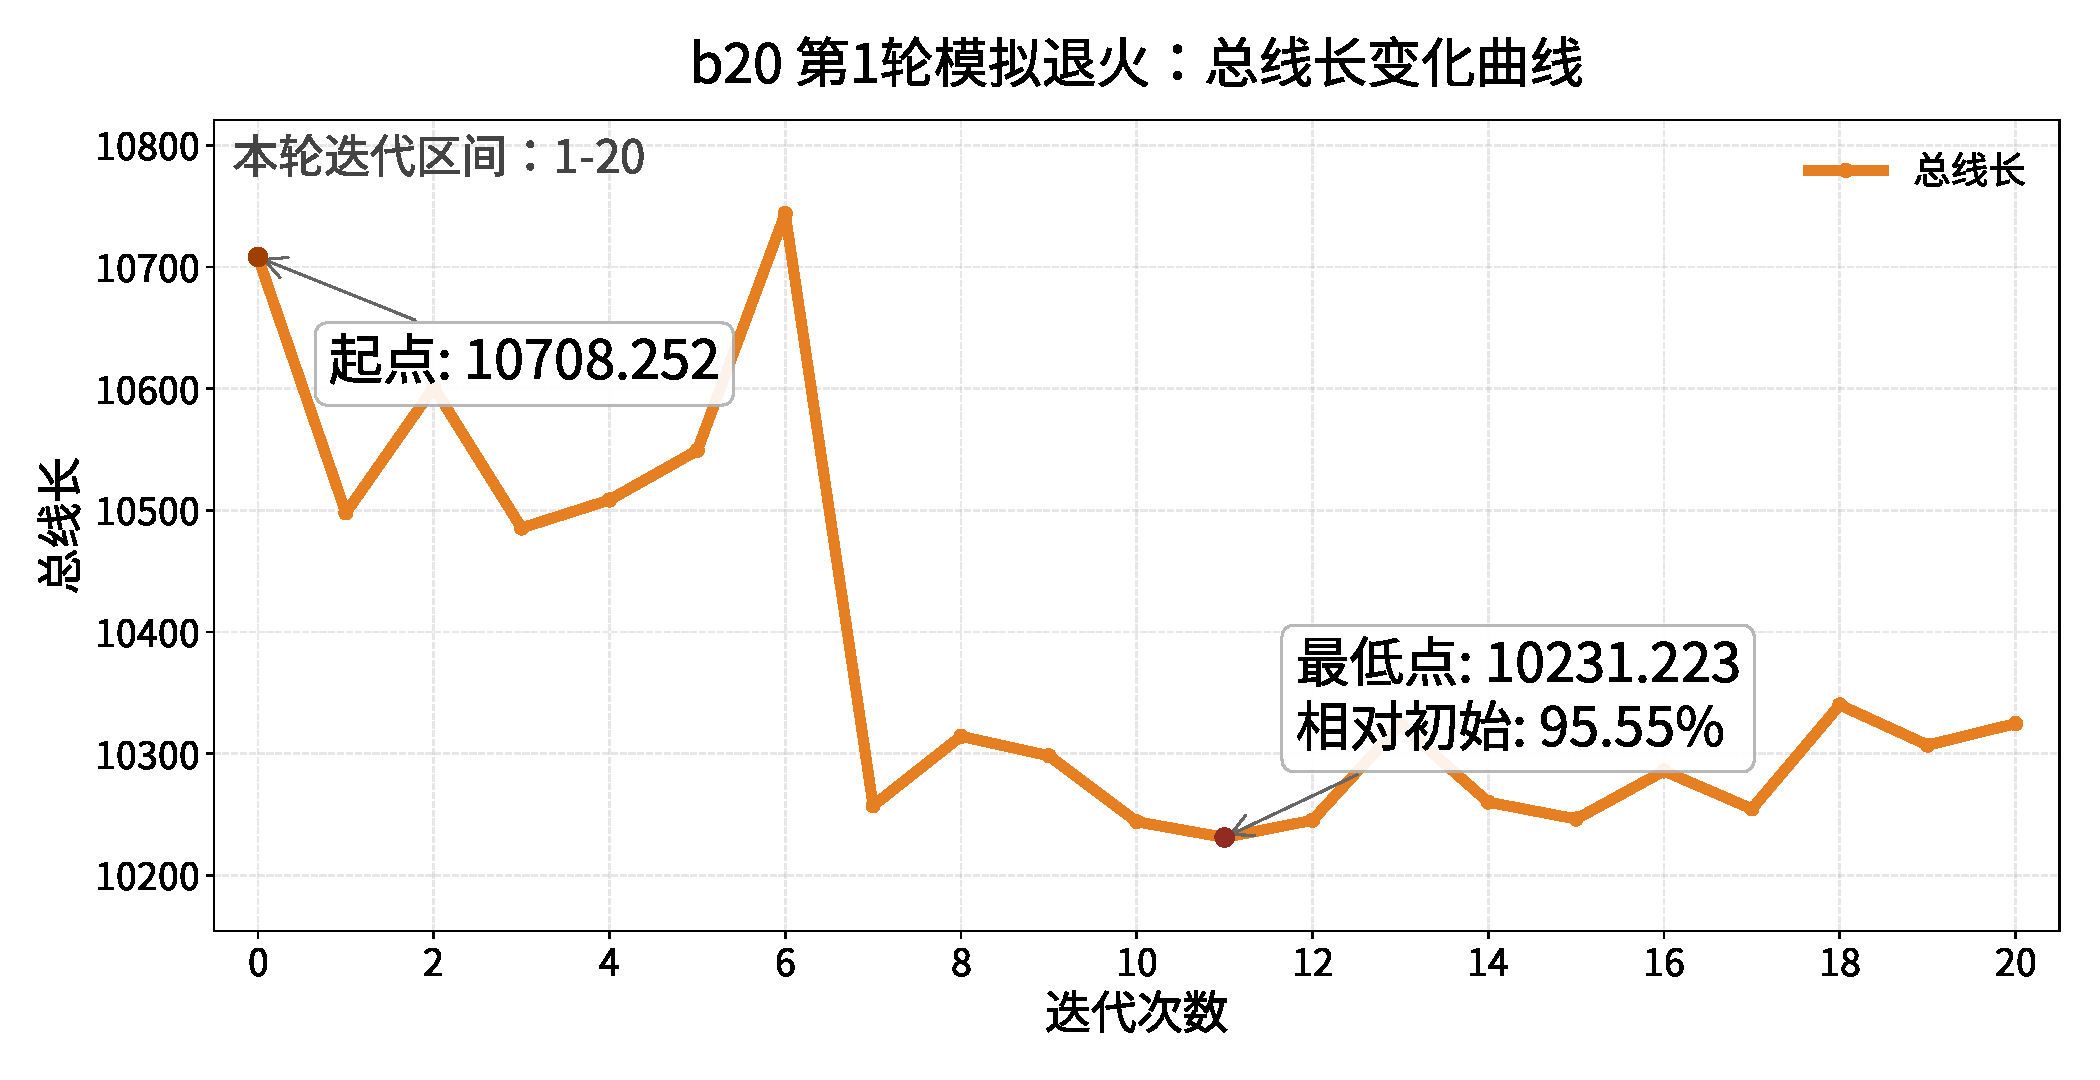
\includegraphics[width=0.96\textwidth]{image/chap04/result/sa_curve_b20/chap4_b20_sa_round1_curve.pdf}
    \caption{\texttt{b20} 第 1 轮模拟退火优化曲线（总线长）}
    \label{fig:chap4-sa-b20-round1-curve}
\end{figure}

第 2 轮曲线（图~\ref{fig:chap4-sa-b20-round2-curve}）以第 1 轮当前最优解为新起点继续搜索，很显然这轮模拟退火更加吃力，整体呈现很难找到比初值好的情况，并在迭代 40 处达到该轮最低值 10167.945（相对轮内起点 99.38\%）。正是这种优化越来越难的情况，因此本章选择使用多段模拟退火来作为优化的策略。
模拟退火中若偶然陷入了局部最优，单纯增加迭代的轮数是很难高效地进行优化的。更稳定的策略是重置某一次解为初始解，然后在已有较优解附近挖掘增量改进空间。

\begin{figure}[!htbp]
    \centering
    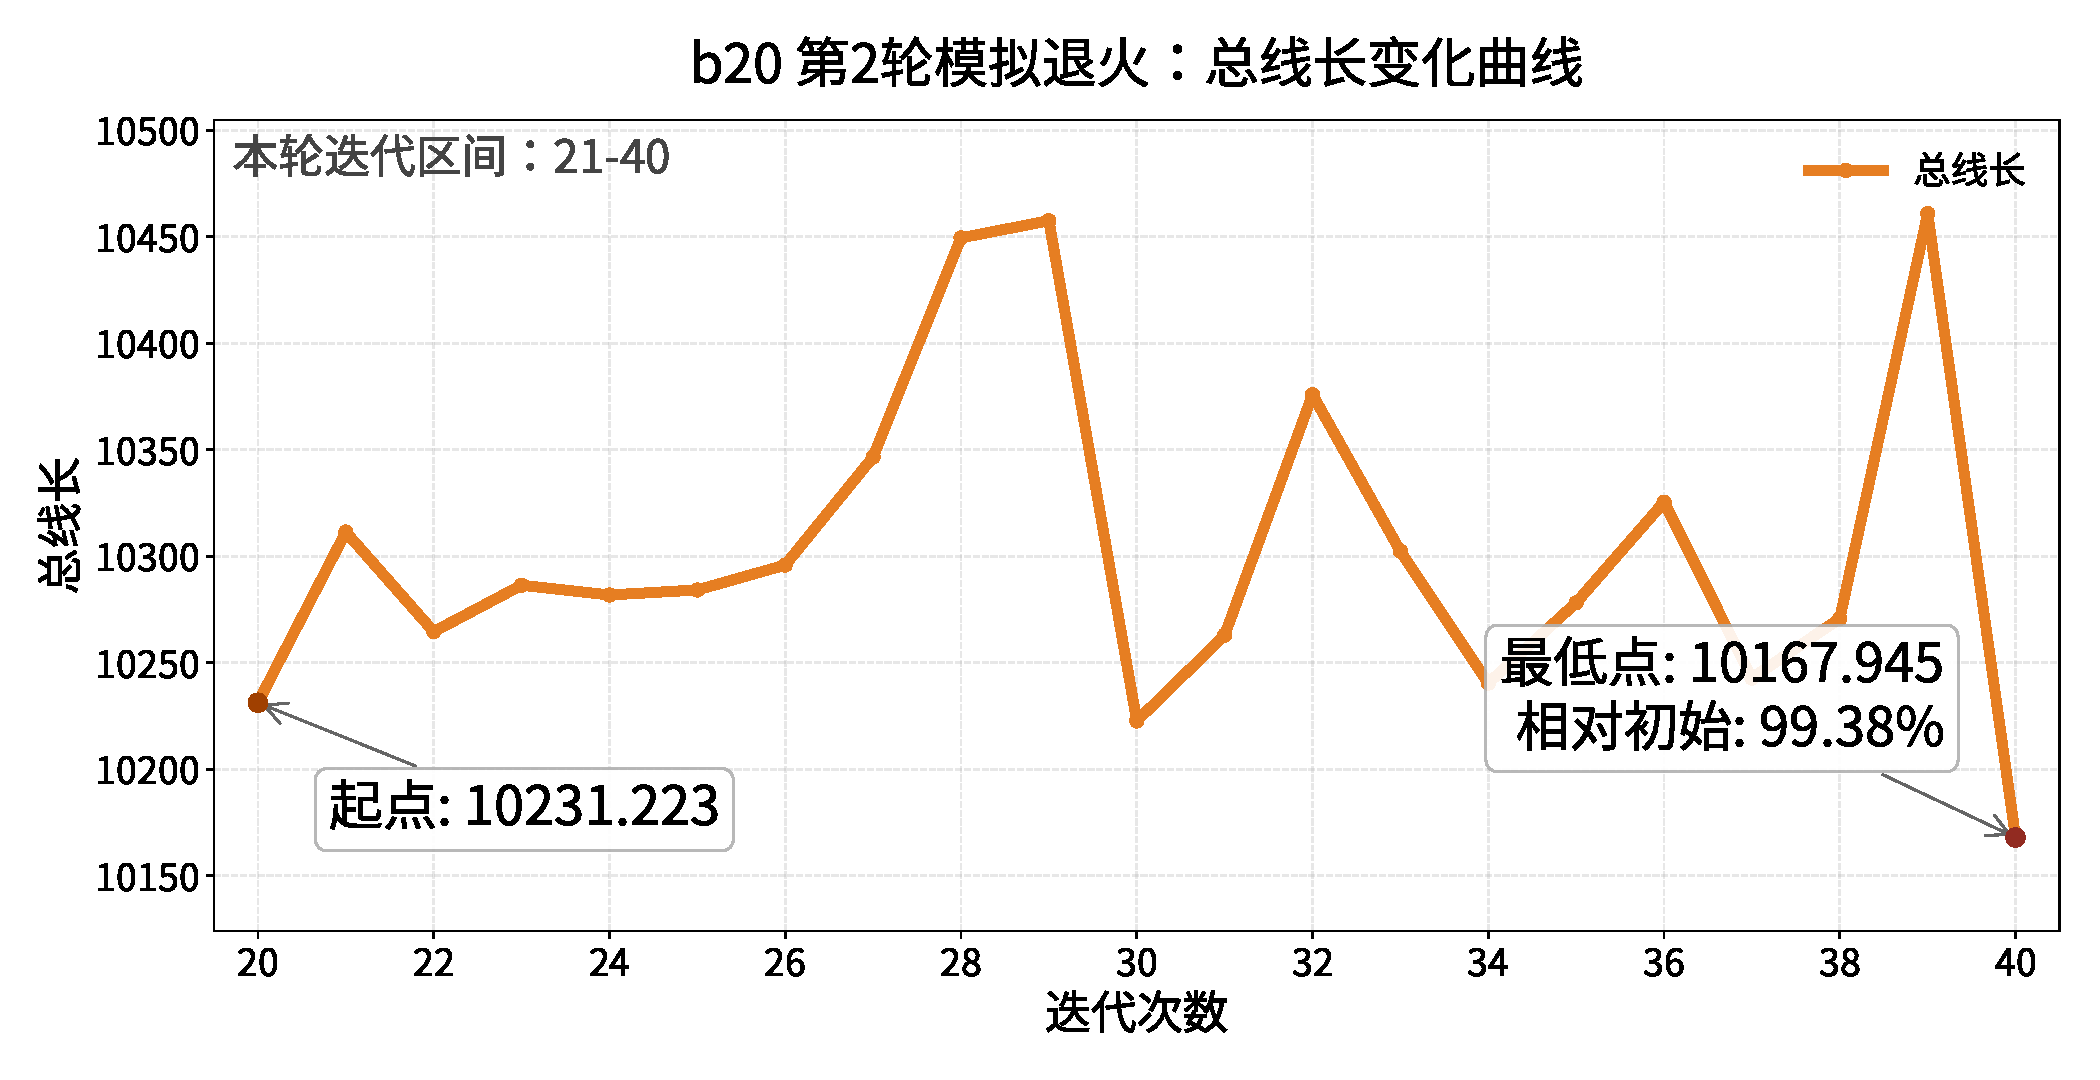
\includegraphics[width=0.96\textwidth]{image/chap04/result/sa_curve_b20/chap4_b20_sa_round2_curve.pdf}
    \caption{\texttt{b20} 第 2 轮模拟退火优化曲线（总线长）}
    \label{fig:chap4-sa-b20-round2-curve}
\end{figure}

综合两轮曲线可见，多段模拟退火在设计合理邻域扰动以及高效阶段性重置初始起点的协同机制下，能够较为有效地推动目标函数向更优方向收敛，验证了本章细粒度引导优化流程在实际运行过程中的有效性。

\subsection{优化前后布局密度与密度方差对比}
\label{sec:chap4-exp-density-variance}

除了以上分析，本文进一步对比了优化前后布局密度分布的统计差异。具体地，对每个测试样例提取优化前与优化后（线长最优迭代）的两组数据，分别统计密度与密度标准差并绘制柱状对比图。

在布局问题中，密度分布会间接影响总线长、通孔数以及可布线性等综合指标：若局部区域过于密集而其他区域过于疏松，可能在统计意义上缩短部分互连路径，从而带来线长下降。因此，本节引入密度相关分析的核心目的，是验证本章线长优化收益是否主要来自这种密度改变效应。

本文对比了优化前与优化后（表~\ref{tab:chap4-sa-before-after} 中对应的最优迭代次），并分别统计密度与密度标准差。若线长收益主要来自密度改变，则通常会表现为平均密度显著变化或密度标准差成倍上升。

图~\ref{fig:chap4-avg-density-before-after} 展示了各测试样例优化前后 \texttt{Density(\%)} 的对比结果，并在最右侧给出了整体均值柱。可以看到，整体平均密度由 70.86\% 提升至 70.87\%，变化幅度极小，说明优化后密度水平整体保持恒定。

\begin{figure}[!htbp]
    \centering
    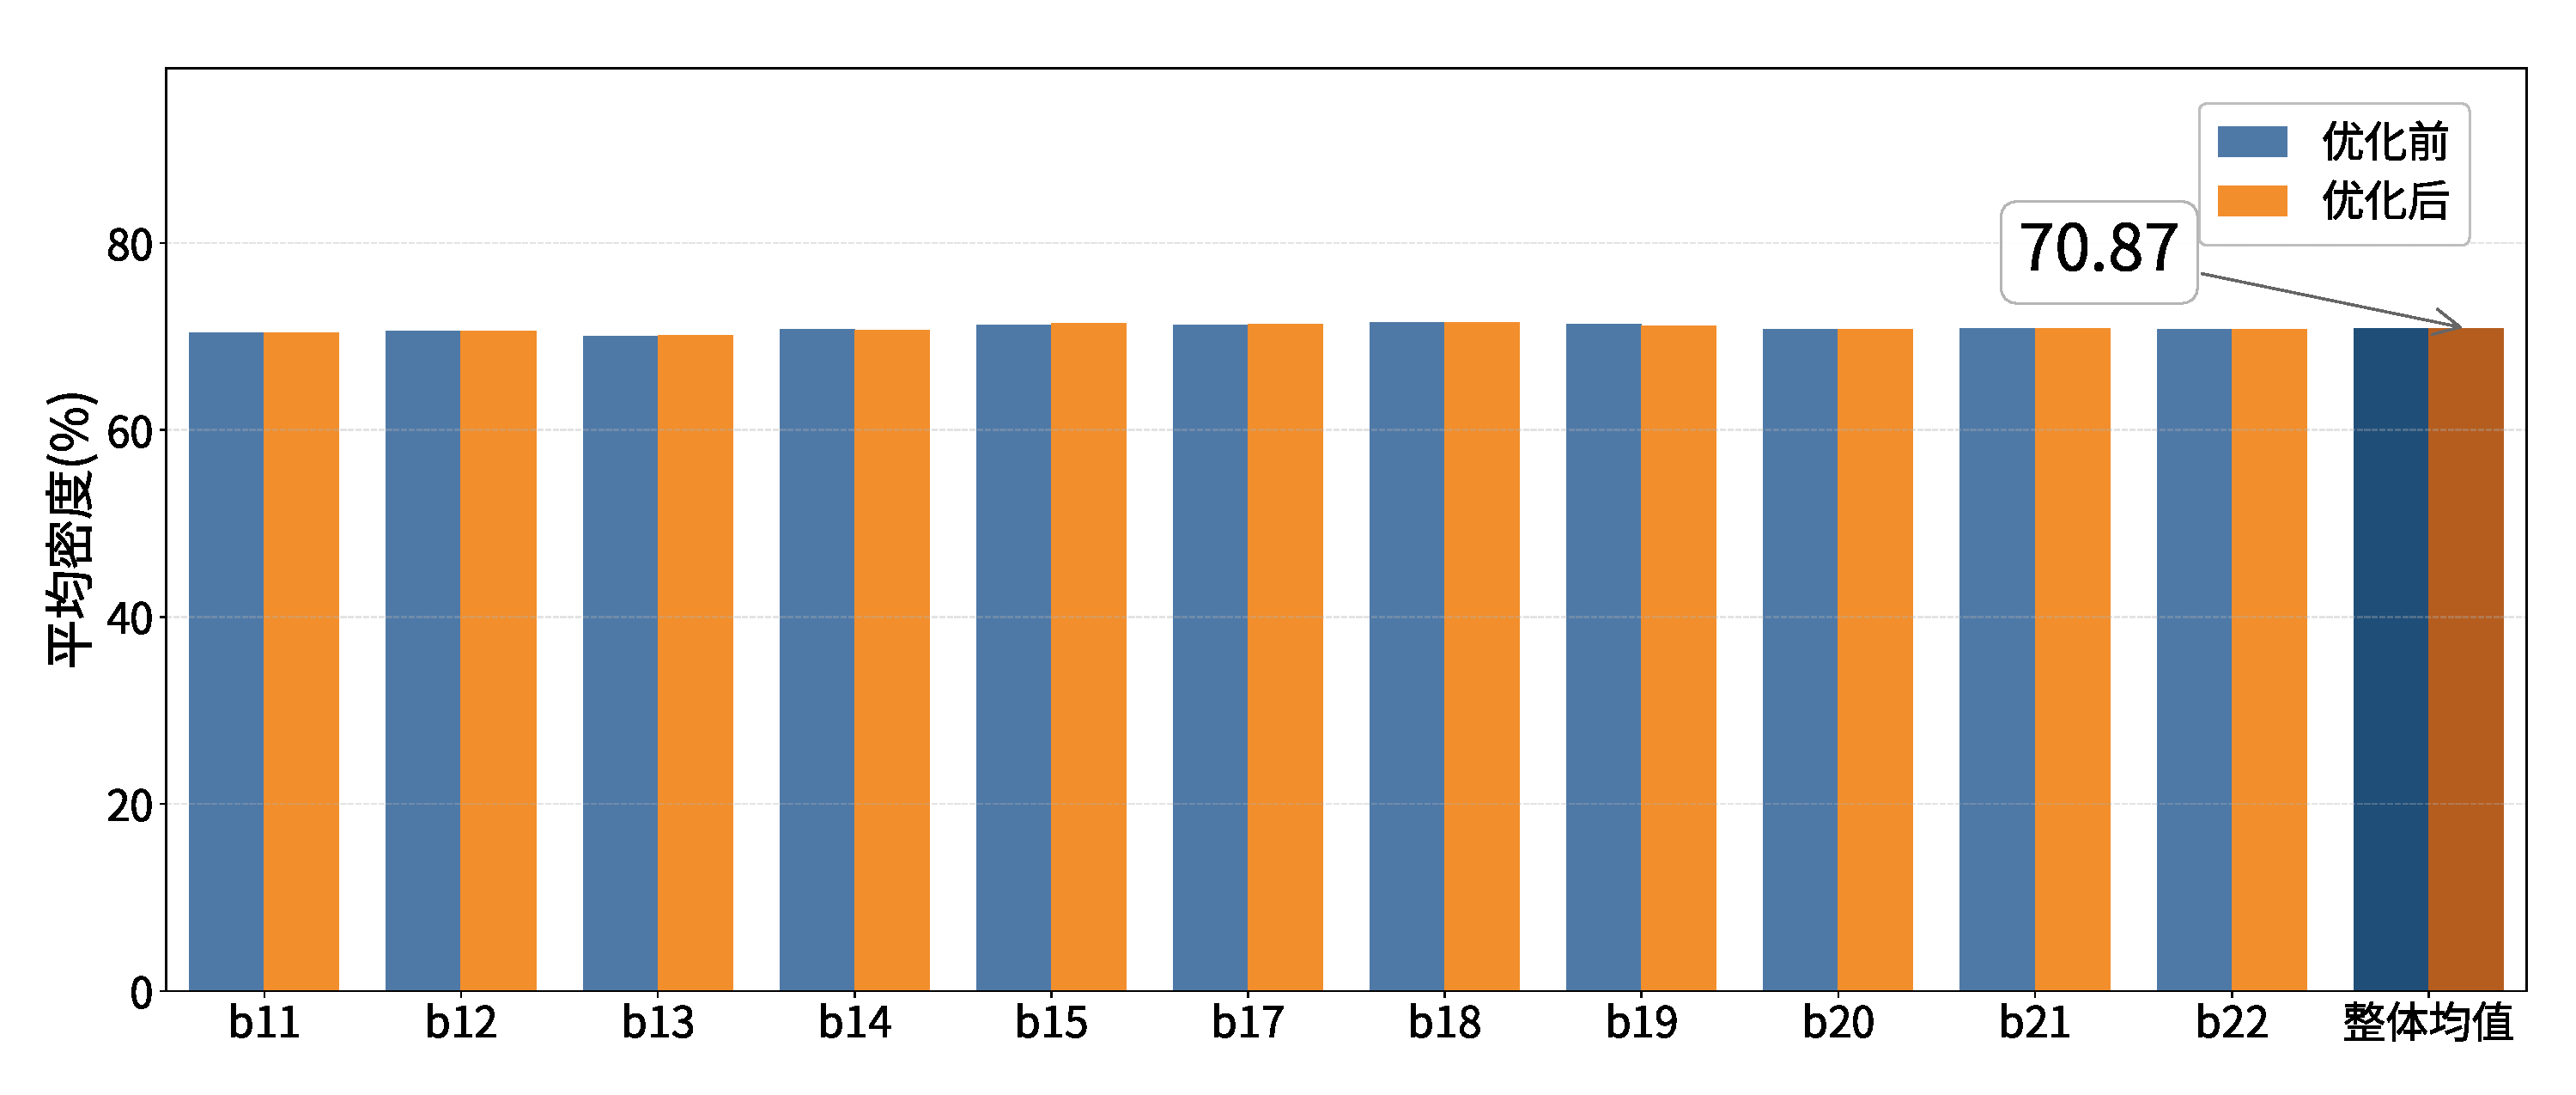
\includegraphics[width=0.98\textwidth]{image/chap04/result/chap4_avg_density_before_after.pdf}
    \caption{各测试样例优化前后密度（Density(\%)）对比（含整体均值）}
    \label{fig:chap4-avg-density-before-after}
\end{figure}

图~\ref{fig:chap4-density-std-before-after} 给出了密度标准差的相对变化结果：将各 case 的优化前标准差统一归一化为 100\%，优化后以相对比例展示，并在最右侧增加整体均值柱。其中，各 case 的优化后数据与表~\ref{tab:chap4-sa-before-after} 的最优迭代次的测试一一对照；整体柱采用原始标准差的加权相对值，结果为 117.9\%，即相较优化前整体增加约 17.9\%。

\begin{figure}[!htbp]
    \centering
    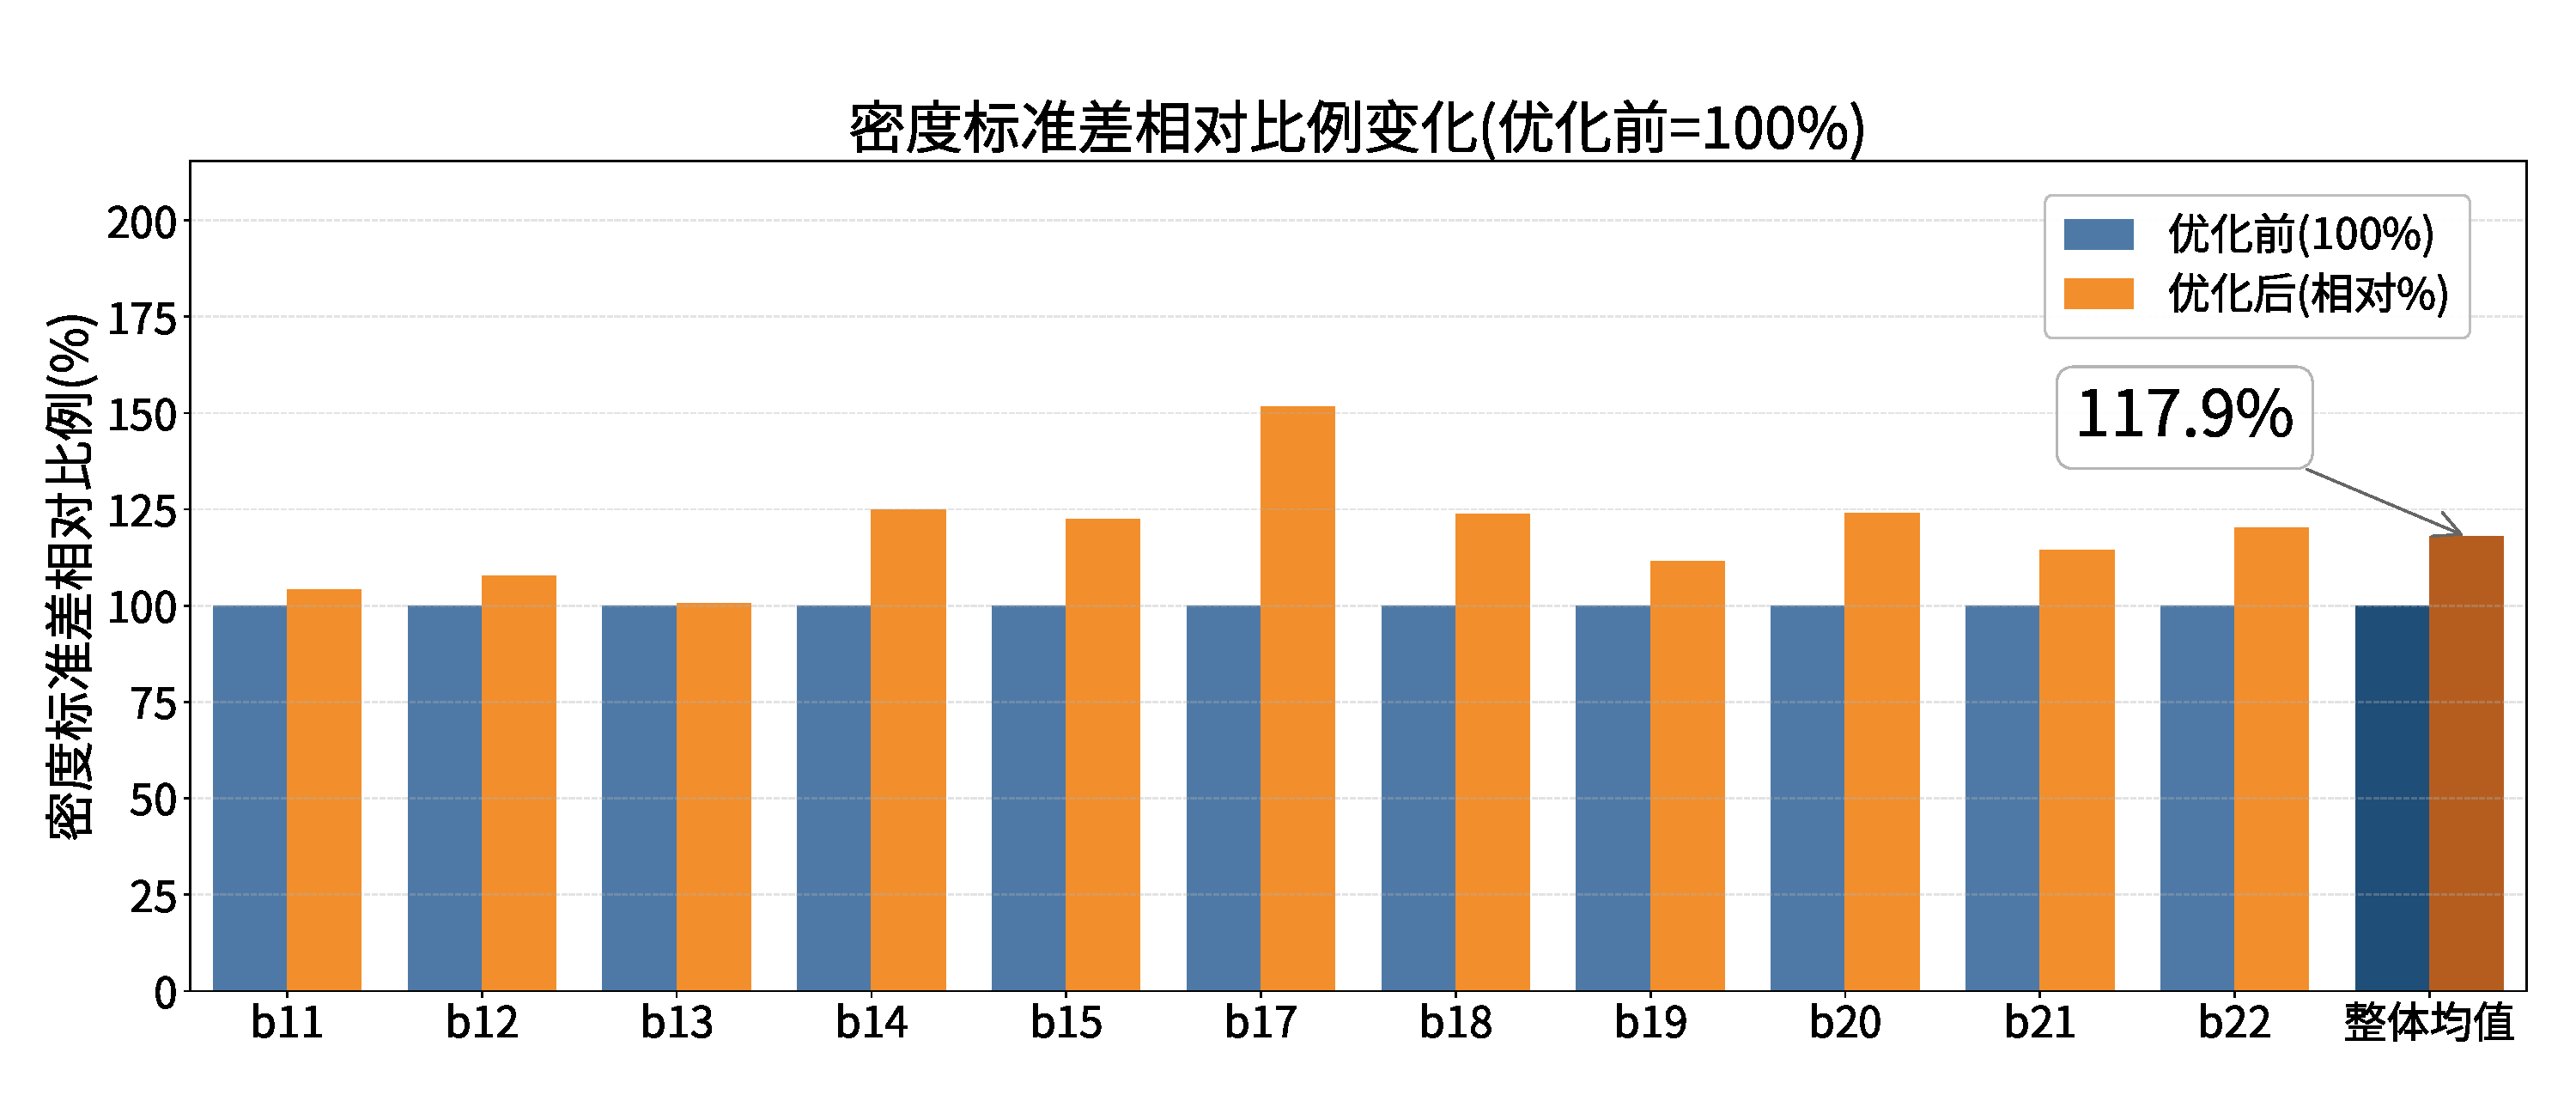
\includegraphics[width=0.98\textwidth]{image/chap04/result/chap4_density_std_before_after.pdf}
    \caption{各测试样例优化前后密度标准差相对变化（优化前归一化为 100\%，含整体均值）}
    \label{fig:chap4-density-std-before-after}
\end{figure}

综合图~\ref{fig:chap4-avg-density-before-after}、图~\ref{fig:chap4-density-std-before-after} 与表~\ref{tab:chap4-sa-before-after} 可见：在平均密度基本持平、密度标准差总体仅有限增长（117.9\%）的情况下，线长仍实现了 3.86\% 的平均优化。这说明本章方法的主要收益并非依赖显著改变密度分布，而是来自细粒度约束引导与多段模拟退火搜索本身。

\section{本章小结}
\label{sec:chap4-summary}

本章围绕解析式粗粒度模块级布局规划结果进一步通过细粒度设计空间探索获得后端收益的课题，提出了基于多段模拟退火的模块级布局细粒度设计空间探索流程。针对仅依赖粗粒度结果可调空间不足、仅依赖纯模拟退火全空间搜索计算开销过高的矛盾，本文给出了基于已有模块级布局结果再进行细粒度布局优化的策略，并在此基础上采用了合理邻域扰动设置，阶段性重置等策略，构建了多段模拟退火的优化流程。

实验结果表明，在11个ITC'99测试样例上，该流程平均实现3.86\%的线长优化，WNS与TNS均满足时序设计要求，密度标准差有小幅增加，平均密度基本持平。案例可视化、退火迭代曲线与密度统计分析三方面结论相互印证，验证了本章方法在布局结果质量上改进的有效性.

